\documentclass[twoside]{book}

% Packages required by doxygen
\usepackage{fixltx2e}
\usepackage{calc}
\usepackage{doxygen}
\usepackage[export]{adjustbox} % also loads graphicx
\usepackage{graphicx}
\usepackage[utf8]{inputenc}
\usepackage{makeidx}
\usepackage{multicol}
\usepackage{multirow}
\PassOptionsToPackage{warn}{textcomp}
\usepackage{textcomp}
\usepackage[nointegrals]{wasysym}
\usepackage[table]{xcolor}

% Font selection
\usepackage[T1]{fontenc}
\usepackage[scaled=.90]{helvet}
\usepackage{courier}
\usepackage{amssymb}
\usepackage{sectsty}
\renewcommand{\familydefault}{\sfdefault}
\allsectionsfont{%
  \fontseries{bc}\selectfont%
  \color{darkgray}%
}
\renewcommand{\DoxyLabelFont}{%
  \fontseries{bc}\selectfont%
  \color{darkgray}%
}
\newcommand{\+}{\discretionary{\mbox{\scriptsize$\hookleftarrow$}}{}{}}

% Page & text layout
\usepackage{geometry}
\geometry{%
  a4paper,%
  top=2.5cm,%
  bottom=2.5cm,%
  left=2.5cm,%
  right=2.5cm%
}
\tolerance=750
\hfuzz=15pt
\hbadness=750
\setlength{\emergencystretch}{15pt}
\setlength{\parindent}{0cm}
\setlength{\parskip}{3ex plus 2ex minus 2ex}
\makeatletter
\renewcommand{\paragraph}{%
  \@startsection{paragraph}{4}{0ex}{-1.0ex}{1.0ex}{%
    \normalfont\normalsize\bfseries\SS@parafont%
  }%
}
\renewcommand{\subparagraph}{%
  \@startsection{subparagraph}{5}{0ex}{-1.0ex}{1.0ex}{%
    \normalfont\normalsize\bfseries\SS@subparafont%
  }%
}
\makeatother

% Headers & footers
\usepackage{fancyhdr}
\pagestyle{fancyplain}
\fancyhead[LE]{\fancyplain{}{\bfseries\thepage}}
\fancyhead[CE]{\fancyplain{}{}}
\fancyhead[RE]{\fancyplain{}{\bfseries\leftmark}}
\fancyhead[LO]{\fancyplain{}{\bfseries\rightmark}}
\fancyhead[CO]{\fancyplain{}{}}
\fancyhead[RO]{\fancyplain{}{\bfseries\thepage}}
\fancyfoot[LE]{\fancyplain{}{}}
\fancyfoot[CE]{\fancyplain{}{}}
\fancyfoot[RE]{\fancyplain{}{\bfseries\scriptsize Generated by Doxygen }}
\fancyfoot[LO]{\fancyplain{}{\bfseries\scriptsize Generated by Doxygen }}
\fancyfoot[CO]{\fancyplain{}{}}
\fancyfoot[RO]{\fancyplain{}{}}
\renewcommand{\footrulewidth}{0.4pt}
\renewcommand{\chaptermark}[1]{%
  \markboth{#1}{}%
}
\renewcommand{\sectionmark}[1]{%
  \markright{\thesection\ #1}%
}

% Indices & bibliography
\usepackage{natbib}
\usepackage[titles]{tocloft}
\setcounter{tocdepth}{3}
\setcounter{secnumdepth}{5}
\makeindex

% Hyperlinks (required, but should be loaded last)
\usepackage{ifpdf}
\ifpdf
  \usepackage[pdftex,pagebackref=true]{hyperref}
\else
  \usepackage[ps2pdf,pagebackref=true]{hyperref}
\fi
\hypersetup{%
  colorlinks=true,%
  linkcolor=blue,%
  citecolor=blue,%
  unicode%
}

% Custom commands
\newcommand{\clearemptydoublepage}{%
  \newpage{\pagestyle{empty}\cleardoublepage}%
}

\usepackage{caption}
\captionsetup{labelsep=space,justification=centering,font={bf},singlelinecheck=off,skip=4pt,position=top}

%===== C O N T E N T S =====

\begin{document}

% Titlepage & ToC
\hypersetup{pageanchor=false,
             bookmarksnumbered=true,
             pdfencoding=unicode
            }
\pagenumbering{alph}
\begin{titlepage}
\vspace*{7cm}
\begin{center}%
{\Large Turtle\+S\+DK }\\
\vspace*{1cm}
{\large Generated by Doxygen 1.8.13}\\
\end{center}
\end{titlepage}
\clearemptydoublepage
\pagenumbering{roman}
\tableofcontents
\clearemptydoublepage
\pagenumbering{arabic}
\hypersetup{pageanchor=true}

%--- Begin generated contents ---
\chapter{Hierarchical Index}
\section{Class Hierarchy}
This inheritance list is sorted roughly, but not completely, alphabetically\+:\begin{DoxyCompactList}
\item \contentsline{section}{Camera}{\pageref{classCamera}}{}
\begin{DoxyCompactList}
\item \contentsline{section}{F\+P\+S\+Camera}{\pageref{classFPSCamera}}{}
\item \contentsline{section}{Orbit\+Camera}{\pageref{classOrbitCamera}}{}
\end{DoxyCompactList}
\item \contentsline{section}{Grid}{\pageref{classGrid}}{}
\item \contentsline{section}{Grid\+Generator}{\pageref{classGridGenerator}}{}
\item \contentsline{section}{Light}{\pageref{classLight}}{}
\begin{DoxyCompactList}
\item \contentsline{section}{Direction\+Light}{\pageref{classDirectionLight}}{}
\item \contentsline{section}{Point\+Light}{\pageref{classPointLight}}{}
\begin{DoxyCompactList}
\item \contentsline{section}{Spot\+Light}{\pageref{classSpotLight}}{}
\end{DoxyCompactList}
\end{DoxyCompactList}
\item \contentsline{section}{Mesh}{\pageref{classMesh}}{}
\item \contentsline{section}{Model}{\pageref{classModel}}{}
\begin{DoxyCompactList}
\item \contentsline{section}{Terrain}{\pageref{classTerrain}}{}
\end{DoxyCompactList}
\item \contentsline{section}{Object}{\pageref{classObject}}{}
\item \contentsline{section}{Shader}{\pageref{classShader}}{}
\item \contentsline{section}{Sky\+Box}{\pageref{classSkyBox}}{}
\item \contentsline{section}{Texture}{\pageref{structTexture}}{}
\item \contentsline{section}{Turtle}{\pageref{classTurtle}}{}
\item \contentsline{section}{Vertex}{\pageref{structVertex}}{}
\end{DoxyCompactList}

\chapter{Class Index}
\section{Class List}
Here are the classes, structs, unions and interfaces with brief descriptions\+:\begin{DoxyCompactList}
\item\contentsline{section}{\hyperlink{classCamera}{Camera} \\*\hyperlink{classCamera}{Camera} used to navigate in a scene }{\pageref{classCamera}}{}
\item\contentsline{section}{\hyperlink{classDirectionLight}{Direction\+Light} }{\pageref{classDirectionLight}}{}
\item\contentsline{section}{\hyperlink{classFPSCamera}{F\+P\+S\+Camera} \\*\hyperlink{classCamera}{Camera} used to navigate in a scene }{\pageref{classFPSCamera}}{}
\item\contentsline{section}{\hyperlink{classGrid}{Grid} \\*A point grid }{\pageref{classGrid}}{}
\item\contentsline{section}{\hyperlink{classGridGenerator}{Grid\+Generator} \\*\hyperlink{classGrid}{Grid} generator }{\pageref{classGridGenerator}}{}
\item\contentsline{section}{\hyperlink{classLight}{Light} }{\pageref{classLight}}{}
\item\contentsline{section}{\hyperlink{classMesh}{Mesh} \\*\hyperlink{classMesh}{Mesh} wrapper }{\pageref{classMesh}}{}
\item\contentsline{section}{\hyperlink{classModel}{Model} \\*A set of one or more mesh }{\pageref{classModel}}{}
\item\contentsline{section}{\hyperlink{classObject}{Object} \\*Wrapper of a model Can be positioned in the spaces Usefulle when creating instances, avoid to duplicate the model }{\pageref{classObject}}{}
\item\contentsline{section}{\hyperlink{classOrbitCamera}{Orbit\+Camera} \\*\hyperlink{classCamera}{Camera} used to rotate around a round-\/shaped object }{\pageref{classOrbitCamera}}{}
\item\contentsline{section}{\hyperlink{classPointLight}{Point\+Light} }{\pageref{classPointLight}}{}
\item\contentsline{section}{\hyperlink{classShader}{Shader} }{\pageref{classShader}}{}
\item\contentsline{section}{\hyperlink{classSkyBox}{Sky\+Box} \\*A Cubemap }{\pageref{classSkyBox}}{}
\item\contentsline{section}{\hyperlink{classSpotLight}{Spot\+Light} }{\pageref{classSpotLight}}{}
\item\contentsline{section}{\hyperlink{classTerrain}{Terrain} \\*A \hyperlink{classTerrain}{Terrain} }{\pageref{classTerrain}}{}
\item\contentsline{section}{\hyperlink{structTexture}{Texture} }{\pageref{structTexture}}{}
\item\contentsline{section}{\hyperlink{classTurtle}{Turtle} \\*Unique instance of the main turtle application. Group everything required to make turtle work }{\pageref{classTurtle}}{}
\item\contentsline{section}{\hyperlink{structVertex}{Vertex} }{\pageref{structVertex}}{}
\end{DoxyCompactList}

\chapter{File Index}
\section{File List}
Here is a list of all files with brief descriptions\+:\begin{DoxyCompactList}
\item\contentsline{section}{src/\hyperlink{camera_8cpp}{camera.\+cpp} }{\pageref{camera_8cpp}}{}
\item\contentsline{section}{src/\hyperlink{camera_8h}{camera.\+h} }{\pageref{camera_8h}}{}
\item\contentsline{section}{src/\hyperlink{fpsCamera_8cpp}{fps\+Camera.\+cpp} }{\pageref{fpsCamera_8cpp}}{}
\item\contentsline{section}{src/\hyperlink{fpsCamera_8h}{fps\+Camera.\+h} }{\pageref{fpsCamera_8h}}{}
\item\contentsline{section}{src/\hyperlink{grid_8cpp}{grid.\+cpp} }{\pageref{grid_8cpp}}{}
\item\contentsline{section}{src/\hyperlink{grid_8h}{grid.\+h} }{\pageref{grid_8h}}{}
\item\contentsline{section}{src/\hyperlink{light_8cpp}{light.\+cpp} }{\pageref{light_8cpp}}{}
\item\contentsline{section}{src/\hyperlink{light_8h}{light.\+h} }{\pageref{light_8h}}{}
\item\contentsline{section}{src/\hyperlink{main_8cpp}{main.\+cpp} }{\pageref{main_8cpp}}{}
\item\contentsline{section}{src/\hyperlink{mesh_8cpp}{mesh.\+cpp} }{\pageref{mesh_8cpp}}{}
\item\contentsline{section}{src/\hyperlink{mesh_8h}{mesh.\+h} }{\pageref{mesh_8h}}{}
\item\contentsline{section}{src/\hyperlink{model_8cpp}{model.\+cpp} }{\pageref{model_8cpp}}{}
\item\contentsline{section}{src/\hyperlink{model_8h}{model.\+h} }{\pageref{model_8h}}{}
\item\contentsline{section}{src/\hyperlink{object_8cpp}{object.\+cpp} }{\pageref{object_8cpp}}{}
\item\contentsline{section}{src/\hyperlink{object_8h}{object.\+h} }{\pageref{object_8h}}{}
\item\contentsline{section}{src/\hyperlink{orbitCamera_8cpp}{orbit\+Camera.\+cpp} }{\pageref{orbitCamera_8cpp}}{}
\item\contentsline{section}{src/\hyperlink{orbitCamera_8h}{orbit\+Camera.\+h} }{\pageref{orbitCamera_8h}}{}
\item\contentsline{section}{src/\hyperlink{shader_8cpp}{shader.\+cpp} }{\pageref{shader_8cpp}}{}
\item\contentsline{section}{src/\hyperlink{shader_8h}{shader.\+h} }{\pageref{shader_8h}}{}
\item\contentsline{section}{src/\hyperlink{skybox_8cpp}{skybox.\+cpp} }{\pageref{skybox_8cpp}}{}
\item\contentsline{section}{src/\hyperlink{skybox_8h}{skybox.\+h} }{\pageref{skybox_8h}}{}
\item\contentsline{section}{src/\hyperlink{terrain_8cpp}{terrain.\+cpp} }{\pageref{terrain_8cpp}}{}
\item\contentsline{section}{src/\hyperlink{terrain_8h}{terrain.\+h} }{\pageref{terrain_8h}}{}
\item\contentsline{section}{src/\hyperlink{turtle_8cpp}{turtle.\+cpp} }{\pageref{turtle_8cpp}}{}
\item\contentsline{section}{src/\hyperlink{turtle_8h}{turtle.\+h} }{\pageref{turtle_8h}}{}
\end{DoxyCompactList}

\chapter{Class Documentation}
\hypertarget{classCamera}{}\section{Camera Class Reference}
\label{classCamera}\index{Camera@{Camera}}


\hyperlink{classCamera}{Camera} used to navigate in a scene.  




{\ttfamily \#include $<$camera.\+h$>$}

Inheritance diagram for Camera\+:\begin{figure}[H]
\begin{center}
\leavevmode
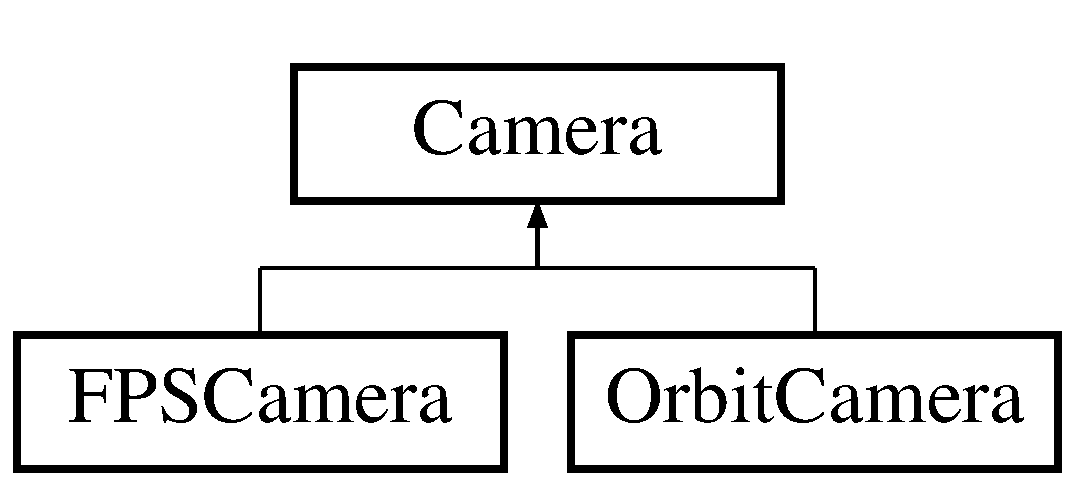
\includegraphics[height=2.000000cm]{classCamera}
\end{center}
\end{figure}
\subsection*{Public Member Functions}
\begin{DoxyCompactItemize}
\item 
virtual void \hyperlink{classCamera_aa7695a960438e5571e14f50ed69f6623}{reset} ()=0
\begin{DoxyCompactList}\small\item\em Reset the camera values. \end{DoxyCompactList}\item 
virtual void \hyperlink{classCamera_abb67395d3094b766d86ad17cedc054c3}{process\+\_\+mouse\+\_\+move} (G\+L\+F\+Wwindow $\ast$window, double xpos, double ypos)
\item 
virtual void \hyperlink{classCamera_affd5e8a22d61e945ba56d2a807b98e61}{process\+\_\+mouse\+\_\+action} (G\+L\+F\+Wwindow $\ast$window, int button, int action, int mods)
\item 
virtual void \hyperlink{classCamera_ac13cc5fa7a3a5c40e53d95e987c1ff04}{process\+\_\+scroll} (G\+L\+F\+Wwindow $\ast$window, double xoffset, double yoffset)
\item 
virtual void \hyperlink{classCamera_ac7fb896a59f9f456ab2041f9dca9b841}{process\+\_\+key} (G\+L\+F\+Wwindow $\ast$, int, int, int, int)
\item 
virtual glm\+::mat4 \hyperlink{classCamera_a279a5a9fdcdb6161bab2c3ff8fce275b}{view} () const =0
\item 
virtual glm\+::mat4 \hyperlink{classCamera_afc206d8b4484d0d8c5e7333b34c68c6f}{projection} () const
\item 
virtual glm\+::vec3 \hyperlink{classCamera_a3ec282533cfc02be93006259d383b6d2}{up} () const =0
\end{DoxyCompactItemize}
\subsection*{Public Attributes}
\begin{DoxyCompactItemize}
\item 
glm\+::vec3 \hyperlink{classCamera_ae54915cea5c8741a9cc38b8f9b6849ff}{pos}
\item 
float \hyperlink{classCamera_aff7393c9cfbccd7e369091f00008da93}{fov} = 0
\end{DoxyCompactItemize}
\subsection*{Protected Attributes}
\begin{DoxyCompactItemize}
\item 
glm\+::vec3 \hyperlink{classCamera_a214af03f2a5040b630f8c24d0952c112}{\+\_\+initial\+Pos} = \{0, 0, 3\}
\item 
float \hyperlink{classCamera_a98641504c424fd46fd742287e8b4c518}{\+\_\+last\+PosX}
\item 
float \hyperlink{classCamera_a5488570163bcbaa8b5c4064d04969806}{\+\_\+last\+PosY}
\item 
bool \hyperlink{classCamera_a4b8929090b9d34548058e10f744f7156}{\+\_\+first\+Move} = true
\end{DoxyCompactItemize}


\subsection{Detailed Description}
\hyperlink{classCamera}{Camera} used to navigate in a scene. 

\subsection{Member Function Documentation}
\mbox{\Hypertarget{classCamera_ac7fb896a59f9f456ab2041f9dca9b841}\label{classCamera_ac7fb896a59f9f456ab2041f9dca9b841}} 
\index{Camera@{Camera}!process\+\_\+key@{process\+\_\+key}}
\index{process\+\_\+key@{process\+\_\+key}!Camera@{Camera}}
\subsubsection{\texorpdfstring{process\+\_\+key()}{process\_key()}}
{\footnotesize\ttfamily void Camera\+::process\+\_\+key (\begin{DoxyParamCaption}\item[{G\+L\+F\+Wwindow $\ast$}]{,  }\item[{int}]{,  }\item[{int}]{,  }\item[{int}]{,  }\item[{int}]{ }\end{DoxyParamCaption})\hspace{0.3cm}{\ttfamily [virtual]}}



Reimplemented in \hyperlink{classFPSCamera_a420a19fa966d3a9caceb81a519419780}{F\+P\+S\+Camera}.

\mbox{\Hypertarget{classCamera_affd5e8a22d61e945ba56d2a807b98e61}\label{classCamera_affd5e8a22d61e945ba56d2a807b98e61}} 
\index{Camera@{Camera}!process\+\_\+mouse\+\_\+action@{process\+\_\+mouse\+\_\+action}}
\index{process\+\_\+mouse\+\_\+action@{process\+\_\+mouse\+\_\+action}!Camera@{Camera}}
\subsubsection{\texorpdfstring{process\+\_\+mouse\+\_\+action()}{process\_mouse\_action()}}
{\footnotesize\ttfamily void Camera\+::process\+\_\+mouse\+\_\+action (\begin{DoxyParamCaption}\item[{G\+L\+F\+Wwindow $\ast$}]{window,  }\item[{int}]{button,  }\item[{int}]{action,  }\item[{int}]{mods }\end{DoxyParamCaption})\hspace{0.3cm}{\ttfamily [virtual]}}



Reimplemented in \hyperlink{classOrbitCamera_af8cb999454725d091971106c4a7bf715}{Orbit\+Camera}.

\mbox{\Hypertarget{classCamera_abb67395d3094b766d86ad17cedc054c3}\label{classCamera_abb67395d3094b766d86ad17cedc054c3}} 
\index{Camera@{Camera}!process\+\_\+mouse\+\_\+move@{process\+\_\+mouse\+\_\+move}}
\index{process\+\_\+mouse\+\_\+move@{process\+\_\+mouse\+\_\+move}!Camera@{Camera}}
\subsubsection{\texorpdfstring{process\+\_\+mouse\+\_\+move()}{process\_mouse\_move()}}
{\footnotesize\ttfamily void Camera\+::process\+\_\+mouse\+\_\+move (\begin{DoxyParamCaption}\item[{G\+L\+F\+Wwindow $\ast$}]{window,  }\item[{double}]{xpos,  }\item[{double}]{ypos }\end{DoxyParamCaption})\hspace{0.3cm}{\ttfamily [virtual]}}



Reimplemented in \hyperlink{classFPSCamera_a3e776ea7816c76d53a0f688c25c4c338}{F\+P\+S\+Camera}, and \hyperlink{classOrbitCamera_a73e280b9244dcbb6b8898a38d0243625}{Orbit\+Camera}.

\mbox{\Hypertarget{classCamera_ac13cc5fa7a3a5c40e53d95e987c1ff04}\label{classCamera_ac13cc5fa7a3a5c40e53d95e987c1ff04}} 
\index{Camera@{Camera}!process\+\_\+scroll@{process\+\_\+scroll}}
\index{process\+\_\+scroll@{process\+\_\+scroll}!Camera@{Camera}}
\subsubsection{\texorpdfstring{process\+\_\+scroll()}{process\_scroll()}}
{\footnotesize\ttfamily void Camera\+::process\+\_\+scroll (\begin{DoxyParamCaption}\item[{G\+L\+F\+Wwindow $\ast$}]{window,  }\item[{double}]{xoffset,  }\item[{double}]{yoffset }\end{DoxyParamCaption})\hspace{0.3cm}{\ttfamily [virtual]}}



Reimplemented in \hyperlink{classFPSCamera_a45640c2e2234cdae4e12bded299e19e8}{F\+P\+S\+Camera}, and \hyperlink{classOrbitCamera_a879faaab86c47e485e119d247279904f}{Orbit\+Camera}.

\mbox{\Hypertarget{classCamera_afc206d8b4484d0d8c5e7333b34c68c6f}\label{classCamera_afc206d8b4484d0d8c5e7333b34c68c6f}} 
\index{Camera@{Camera}!projection@{projection}}
\index{projection@{projection}!Camera@{Camera}}
\subsubsection{\texorpdfstring{projection()}{projection()}}
{\footnotesize\ttfamily glm\+::mat4 Camera\+::projection (\begin{DoxyParamCaption}{ }\end{DoxyParamCaption}) const\hspace{0.3cm}{\ttfamily [virtual]}}

\mbox{\Hypertarget{classCamera_aa7695a960438e5571e14f50ed69f6623}\label{classCamera_aa7695a960438e5571e14f50ed69f6623}} 
\index{Camera@{Camera}!reset@{reset}}
\index{reset@{reset}!Camera@{Camera}}
\subsubsection{\texorpdfstring{reset()}{reset()}}
{\footnotesize\ttfamily virtual void Camera\+::reset (\begin{DoxyParamCaption}{ }\end{DoxyParamCaption})\hspace{0.3cm}{\ttfamily [pure virtual]}}



Reset the camera values. 



Implemented in \hyperlink{classFPSCamera_a5076d0c700255c33daff490d73c77761}{F\+P\+S\+Camera}, and \hyperlink{classOrbitCamera_a022751aa06693232844732adb00e7d71}{Orbit\+Camera}.

\mbox{\Hypertarget{classCamera_a3ec282533cfc02be93006259d383b6d2}\label{classCamera_a3ec282533cfc02be93006259d383b6d2}} 
\index{Camera@{Camera}!up@{up}}
\index{up@{up}!Camera@{Camera}}
\subsubsection{\texorpdfstring{up()}{up()}}
{\footnotesize\ttfamily virtual glm\+::vec3 Camera\+::up (\begin{DoxyParamCaption}{ }\end{DoxyParamCaption}) const\hspace{0.3cm}{\ttfamily [pure virtual]}}



Implemented in \hyperlink{classFPSCamera_a1b6470a9ebb906bc31a2742b943552a1}{F\+P\+S\+Camera}, and \hyperlink{classOrbitCamera_a1d65d137e3ef3f32c3b8eb31b49047fc}{Orbit\+Camera}.

\mbox{\Hypertarget{classCamera_a279a5a9fdcdb6161bab2c3ff8fce275b}\label{classCamera_a279a5a9fdcdb6161bab2c3ff8fce275b}} 
\index{Camera@{Camera}!view@{view}}
\index{view@{view}!Camera@{Camera}}
\subsubsection{\texorpdfstring{view()}{view()}}
{\footnotesize\ttfamily virtual glm\+::mat4 Camera\+::view (\begin{DoxyParamCaption}{ }\end{DoxyParamCaption}) const\hspace{0.3cm}{\ttfamily [pure virtual]}}



Implemented in \hyperlink{classFPSCamera_a41a04414a362e7aa866d490900830cb8}{F\+P\+S\+Camera}, and \hyperlink{classOrbitCamera_a07595f9d11666c180934e47ba8abae73}{Orbit\+Camera}.



\subsection{Member Data Documentation}
\mbox{\Hypertarget{classCamera_a4b8929090b9d34548058e10f744f7156}\label{classCamera_a4b8929090b9d34548058e10f744f7156}} 
\index{Camera@{Camera}!\+\_\+first\+Move@{\+\_\+first\+Move}}
\index{\+\_\+first\+Move@{\+\_\+first\+Move}!Camera@{Camera}}
\subsubsection{\texorpdfstring{\+\_\+first\+Move}{\_firstMove}}
{\footnotesize\ttfamily bool Camera\+::\+\_\+first\+Move = true\hspace{0.3cm}{\ttfamily [protected]}}

\mbox{\Hypertarget{classCamera_a214af03f2a5040b630f8c24d0952c112}\label{classCamera_a214af03f2a5040b630f8c24d0952c112}} 
\index{Camera@{Camera}!\+\_\+initial\+Pos@{\+\_\+initial\+Pos}}
\index{\+\_\+initial\+Pos@{\+\_\+initial\+Pos}!Camera@{Camera}}
\subsubsection{\texorpdfstring{\+\_\+initial\+Pos}{\_initialPos}}
{\footnotesize\ttfamily glm\+::vec3 Camera\+::\+\_\+initial\+Pos = \{0, 0, 3\}\hspace{0.3cm}{\ttfamily [protected]}}

\mbox{\Hypertarget{classCamera_a98641504c424fd46fd742287e8b4c518}\label{classCamera_a98641504c424fd46fd742287e8b4c518}} 
\index{Camera@{Camera}!\+\_\+last\+PosX@{\+\_\+last\+PosX}}
\index{\+\_\+last\+PosX@{\+\_\+last\+PosX}!Camera@{Camera}}
\subsubsection{\texorpdfstring{\+\_\+last\+PosX}{\_lastPosX}}
{\footnotesize\ttfamily float Camera\+::\+\_\+last\+PosX\hspace{0.3cm}{\ttfamily [protected]}}

\mbox{\Hypertarget{classCamera_a5488570163bcbaa8b5c4064d04969806}\label{classCamera_a5488570163bcbaa8b5c4064d04969806}} 
\index{Camera@{Camera}!\+\_\+last\+PosY@{\+\_\+last\+PosY}}
\index{\+\_\+last\+PosY@{\+\_\+last\+PosY}!Camera@{Camera}}
\subsubsection{\texorpdfstring{\+\_\+last\+PosY}{\_lastPosY}}
{\footnotesize\ttfamily float Camera\+::\+\_\+last\+PosY\hspace{0.3cm}{\ttfamily [protected]}}

\mbox{\Hypertarget{classCamera_aff7393c9cfbccd7e369091f00008da93}\label{classCamera_aff7393c9cfbccd7e369091f00008da93}} 
\index{Camera@{Camera}!fov@{fov}}
\index{fov@{fov}!Camera@{Camera}}
\subsubsection{\texorpdfstring{fov}{fov}}
{\footnotesize\ttfamily float Camera\+::fov = 0}

\mbox{\Hypertarget{classCamera_ae54915cea5c8741a9cc38b8f9b6849ff}\label{classCamera_ae54915cea5c8741a9cc38b8f9b6849ff}} 
\index{Camera@{Camera}!pos@{pos}}
\index{pos@{pos}!Camera@{Camera}}
\subsubsection{\texorpdfstring{pos}{pos}}
{\footnotesize\ttfamily glm\+::vec3 Camera\+::pos}



The documentation for this class was generated from the following files\+:\begin{DoxyCompactItemize}
\item 
src/\hyperlink{camera_8h}{camera.\+h}\item 
src/\hyperlink{camera_8cpp}{camera.\+cpp}\end{DoxyCompactItemize}

\hypertarget{classDirectionLight}{}\section{Direction\+Light Class Reference}
\label{classDirectionLight}\index{Direction\+Light@{Direction\+Light}}


{\ttfamily \#include $<$light.\+h$>$}

Inheritance diagram for Direction\+Light\+:\begin{figure}[H]
\begin{center}
\leavevmode
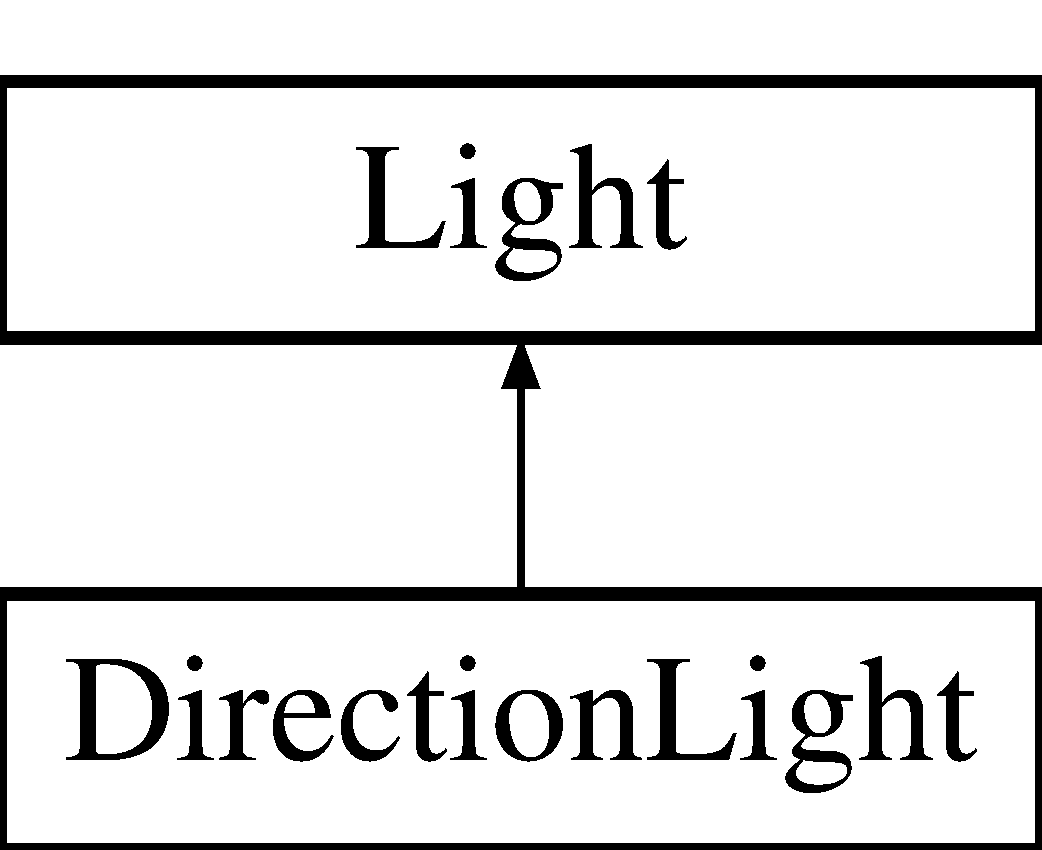
\includegraphics[height=2.000000cm]{classDirectionLight}
\end{center}
\end{figure}
\subsection*{Public Member Functions}
\begin{DoxyCompactItemize}
\item 
virtual void \hyperlink{classDirectionLight_ab10f7b680a8245bd4db3b7340593e485}{set\+Uniforms} (const \hyperlink{classShader}{Shader} \&shader, const std\+::string \&uname) const
\item 
virtual void \hyperlink{classDirectionLight_a85ac86467a3053dea596b0ebf362b68f}{ui} ()
\end{DoxyCompactItemize}
\subsection*{Public Attributes}
\begin{DoxyCompactItemize}
\item 
glm\+::vec3 \hyperlink{classDirectionLight_a838d158caa1ed127775a915ff4506861}{direction\+\_\+} = \{-\/10.f, -\/10.f, -\/10.f\}
\end{DoxyCompactItemize}


\subsection{Member Function Documentation}
\mbox{\Hypertarget{classDirectionLight_ab10f7b680a8245bd4db3b7340593e485}\label{classDirectionLight_ab10f7b680a8245bd4db3b7340593e485}} 
\index{Direction\+Light@{Direction\+Light}!set\+Uniforms@{set\+Uniforms}}
\index{set\+Uniforms@{set\+Uniforms}!Direction\+Light@{Direction\+Light}}
\subsubsection{\texorpdfstring{set\+Uniforms()}{setUniforms()}}
{\footnotesize\ttfamily void Direction\+Light\+::set\+Uniforms (\begin{DoxyParamCaption}\item[{const \hyperlink{classShader}{Shader} \&}]{shader,  }\item[{const std\+::string \&}]{uname }\end{DoxyParamCaption}) const\hspace{0.3cm}{\ttfamily [virtual]}}



Reimplemented from \hyperlink{classLight_adfffa53d21bbeaa638c0bc5ae5a852cc}{Light}.

\mbox{\Hypertarget{classDirectionLight_a85ac86467a3053dea596b0ebf362b68f}\label{classDirectionLight_a85ac86467a3053dea596b0ebf362b68f}} 
\index{Direction\+Light@{Direction\+Light}!ui@{ui}}
\index{ui@{ui}!Direction\+Light@{Direction\+Light}}
\subsubsection{\texorpdfstring{ui()}{ui()}}
{\footnotesize\ttfamily void Direction\+Light\+::ui (\begin{DoxyParamCaption}{ }\end{DoxyParamCaption})\hspace{0.3cm}{\ttfamily [virtual]}}



Reimplemented from \hyperlink{classLight_a15770d3a4b173cd517477dfb5d5bcab9}{Light}.



\subsection{Member Data Documentation}
\mbox{\Hypertarget{classDirectionLight_a838d158caa1ed127775a915ff4506861}\label{classDirectionLight_a838d158caa1ed127775a915ff4506861}} 
\index{Direction\+Light@{Direction\+Light}!direction\+\_\+@{direction\+\_\+}}
\index{direction\+\_\+@{direction\+\_\+}!Direction\+Light@{Direction\+Light}}
\subsubsection{\texorpdfstring{direction\+\_\+}{direction\_}}
{\footnotesize\ttfamily glm\+::vec3 Direction\+Light\+::direction\+\_\+ = \{-\/10.f, -\/10.f, -\/10.f\}}



The documentation for this class was generated from the following files\+:\begin{DoxyCompactItemize}
\item 
src/\hyperlink{light_8h}{light.\+h}\item 
src/\hyperlink{light_8cpp}{light.\+cpp}\end{DoxyCompactItemize}

\hypertarget{classFPSCamera}{}\section{F\+P\+S\+Camera Class Reference}
\label{classFPSCamera}\index{F\+P\+S\+Camera@{F\+P\+S\+Camera}}


\hyperlink{classCamera}{Camera} used to navigate in a scene.  




{\ttfamily \#include $<$fps\+Camera.\+h$>$}

Inheritance diagram for F\+P\+S\+Camera\+:\begin{figure}[H]
\begin{center}
\leavevmode
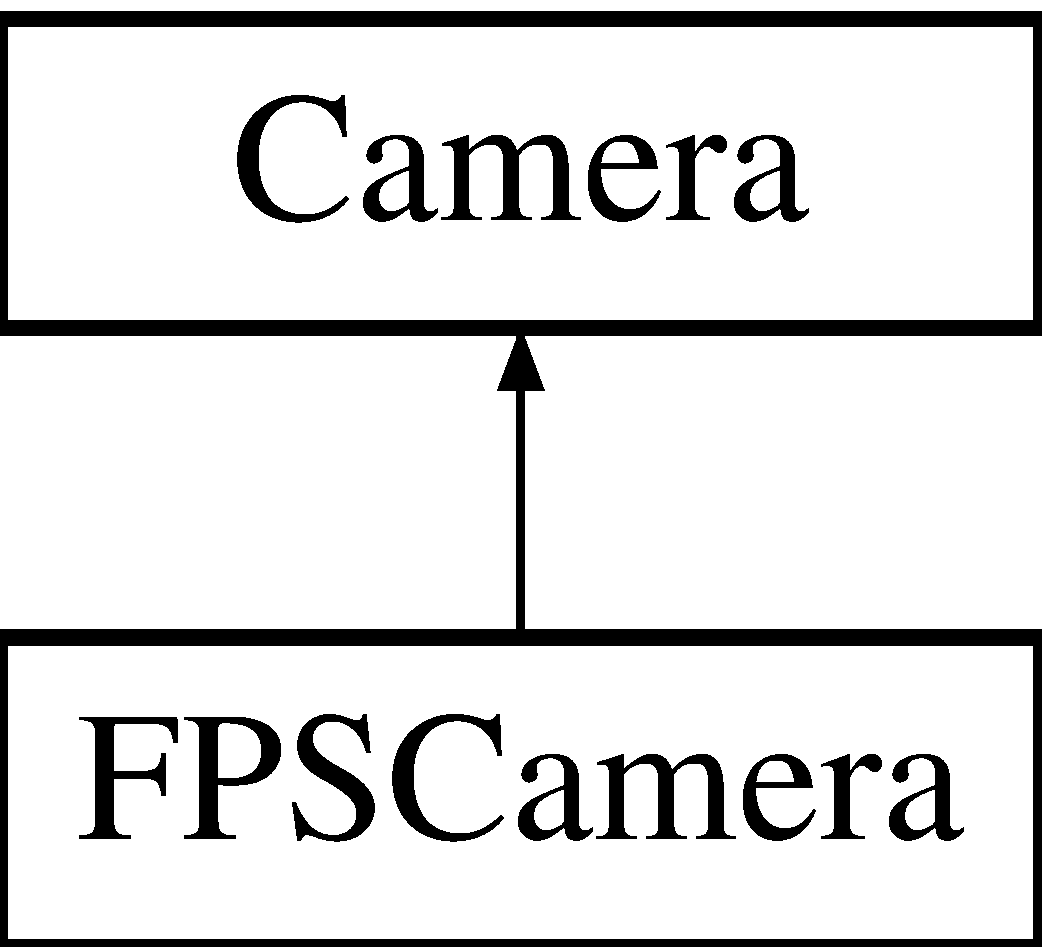
\includegraphics[height=2.000000cm]{classFPSCamera}
\end{center}
\end{figure}
\subsection*{Public Member Functions}
\begin{DoxyCompactItemize}
\item 
\hyperlink{classFPSCamera_a4176f2807be12da32763f66ba55b9621}{F\+P\+S\+Camera} ()
\begin{DoxyCompactList}\small\item\em Create a default fps camera. \end{DoxyCompactList}\item 
void \hyperlink{classFPSCamera_a5076d0c700255c33daff490d73c77761}{reset} ()
\begin{DoxyCompactList}\small\item\em Reset the camera values. \end{DoxyCompactList}\item 
void \hyperlink{classFPSCamera_a3e776ea7816c76d53a0f688c25c4c338}{process\+\_\+mouse\+\_\+move} (G\+L\+F\+Wwindow $\ast$window, double xpos, double ypos)
\item 
void \hyperlink{classFPSCamera_a45640c2e2234cdae4e12bded299e19e8}{process\+\_\+scroll} (G\+L\+F\+Wwindow $\ast$window, double xoffset, double yoffset)
\item 
void \hyperlink{classFPSCamera_a420a19fa966d3a9caceb81a519419780}{process\+\_\+key} (G\+L\+F\+Wwindow $\ast$, int, int, int, int)
\item 
glm\+::mat4 \hyperlink{classFPSCamera_a41a04414a362e7aa866d490900830cb8}{view} () const
\item 
glm\+::vec3 \hyperlink{classFPSCamera_a1b6470a9ebb906bc31a2742b943552a1}{up} () const
\end{DoxyCompactItemize}
\subsection*{Public Attributes}
\begin{DoxyCompactItemize}
\item 
glm\+::vec3 \hyperlink{classFPSCamera_a0f5edc21e058e893866ab7479b275a9a}{cam\+Front}
\item 
glm\+::vec3 \hyperlink{classFPSCamera_aa0ec22bd80a3e35f6b2ae12f830c07c4}{cam\+Up}
\end{DoxyCompactItemize}
\subsection*{Additional Inherited Members}


\subsection{Detailed Description}
\hyperlink{classCamera}{Camera} used to navigate in a scene. 

\subsection{Constructor \& Destructor Documentation}
\mbox{\Hypertarget{classFPSCamera_a4176f2807be12da32763f66ba55b9621}\label{classFPSCamera_a4176f2807be12da32763f66ba55b9621}} 
\index{F\+P\+S\+Camera@{F\+P\+S\+Camera}!F\+P\+S\+Camera@{F\+P\+S\+Camera}}
\index{F\+P\+S\+Camera@{F\+P\+S\+Camera}!F\+P\+S\+Camera@{F\+P\+S\+Camera}}
\subsubsection{\texorpdfstring{F\+P\+S\+Camera()}{FPSCamera()}}
{\footnotesize\ttfamily F\+P\+S\+Camera\+::\+F\+P\+S\+Camera (\begin{DoxyParamCaption}{ }\end{DoxyParamCaption})}



Create a default fps camera. 



\subsection{Member Function Documentation}
\mbox{\Hypertarget{classFPSCamera_a420a19fa966d3a9caceb81a519419780}\label{classFPSCamera_a420a19fa966d3a9caceb81a519419780}} 
\index{F\+P\+S\+Camera@{F\+P\+S\+Camera}!process\+\_\+key@{process\+\_\+key}}
\index{process\+\_\+key@{process\+\_\+key}!F\+P\+S\+Camera@{F\+P\+S\+Camera}}
\subsubsection{\texorpdfstring{process\+\_\+key()}{process\_key()}}
{\footnotesize\ttfamily void F\+P\+S\+Camera\+::process\+\_\+key (\begin{DoxyParamCaption}\item[{G\+L\+F\+Wwindow $\ast$}]{window,  }\item[{int}]{key,  }\item[{int}]{,  }\item[{int}]{action,  }\item[{int}]{moods }\end{DoxyParamCaption})\hspace{0.3cm}{\ttfamily [virtual]}}



Reimplemented from \hyperlink{classCamera_ac7fb896a59f9f456ab2041f9dca9b841}{Camera}.

\mbox{\Hypertarget{classFPSCamera_a3e776ea7816c76d53a0f688c25c4c338}\label{classFPSCamera_a3e776ea7816c76d53a0f688c25c4c338}} 
\index{F\+P\+S\+Camera@{F\+P\+S\+Camera}!process\+\_\+mouse\+\_\+move@{process\+\_\+mouse\+\_\+move}}
\index{process\+\_\+mouse\+\_\+move@{process\+\_\+mouse\+\_\+move}!F\+P\+S\+Camera@{F\+P\+S\+Camera}}
\subsubsection{\texorpdfstring{process\+\_\+mouse\+\_\+move()}{process\_mouse\_move()}}
{\footnotesize\ttfamily void F\+P\+S\+Camera\+::process\+\_\+mouse\+\_\+move (\begin{DoxyParamCaption}\item[{G\+L\+F\+Wwindow $\ast$}]{window,  }\item[{double}]{xpos,  }\item[{double}]{ypos }\end{DoxyParamCaption})\hspace{0.3cm}{\ttfamily [virtual]}}



Reimplemented from \hyperlink{classCamera_abb67395d3094b766d86ad17cedc054c3}{Camera}.

\mbox{\Hypertarget{classFPSCamera_a45640c2e2234cdae4e12bded299e19e8}\label{classFPSCamera_a45640c2e2234cdae4e12bded299e19e8}} 
\index{F\+P\+S\+Camera@{F\+P\+S\+Camera}!process\+\_\+scroll@{process\+\_\+scroll}}
\index{process\+\_\+scroll@{process\+\_\+scroll}!F\+P\+S\+Camera@{F\+P\+S\+Camera}}
\subsubsection{\texorpdfstring{process\+\_\+scroll()}{process\_scroll()}}
{\footnotesize\ttfamily void F\+P\+S\+Camera\+::process\+\_\+scroll (\begin{DoxyParamCaption}\item[{G\+L\+F\+Wwindow $\ast$}]{window,  }\item[{double}]{xoffset,  }\item[{double}]{yoffset }\end{DoxyParamCaption})\hspace{0.3cm}{\ttfamily [virtual]}}



Reimplemented from \hyperlink{classCamera_ac13cc5fa7a3a5c40e53d95e987c1ff04}{Camera}.

\mbox{\Hypertarget{classFPSCamera_a5076d0c700255c33daff490d73c77761}\label{classFPSCamera_a5076d0c700255c33daff490d73c77761}} 
\index{F\+P\+S\+Camera@{F\+P\+S\+Camera}!reset@{reset}}
\index{reset@{reset}!F\+P\+S\+Camera@{F\+P\+S\+Camera}}
\subsubsection{\texorpdfstring{reset()}{reset()}}
{\footnotesize\ttfamily void F\+P\+S\+Camera\+::reset (\begin{DoxyParamCaption}{ }\end{DoxyParamCaption})\hspace{0.3cm}{\ttfamily [virtual]}}



Reset the camera values. 



Implements \hyperlink{classCamera_aa7695a960438e5571e14f50ed69f6623}{Camera}.

\mbox{\Hypertarget{classFPSCamera_a1b6470a9ebb906bc31a2742b943552a1}\label{classFPSCamera_a1b6470a9ebb906bc31a2742b943552a1}} 
\index{F\+P\+S\+Camera@{F\+P\+S\+Camera}!up@{up}}
\index{up@{up}!F\+P\+S\+Camera@{F\+P\+S\+Camera}}
\subsubsection{\texorpdfstring{up()}{up()}}
{\footnotesize\ttfamily glm\+::vec3 F\+P\+S\+Camera\+::up (\begin{DoxyParamCaption}{ }\end{DoxyParamCaption}) const\hspace{0.3cm}{\ttfamily [virtual]}}



Implements \hyperlink{classCamera_a3ec282533cfc02be93006259d383b6d2}{Camera}.

\mbox{\Hypertarget{classFPSCamera_a41a04414a362e7aa866d490900830cb8}\label{classFPSCamera_a41a04414a362e7aa866d490900830cb8}} 
\index{F\+P\+S\+Camera@{F\+P\+S\+Camera}!view@{view}}
\index{view@{view}!F\+P\+S\+Camera@{F\+P\+S\+Camera}}
\subsubsection{\texorpdfstring{view()}{view()}}
{\footnotesize\ttfamily glm\+::mat4 F\+P\+S\+Camera\+::view (\begin{DoxyParamCaption}{ }\end{DoxyParamCaption}) const\hspace{0.3cm}{\ttfamily [virtual]}}



Implements \hyperlink{classCamera_a279a5a9fdcdb6161bab2c3ff8fce275b}{Camera}.



\subsection{Member Data Documentation}
\mbox{\Hypertarget{classFPSCamera_a0f5edc21e058e893866ab7479b275a9a}\label{classFPSCamera_a0f5edc21e058e893866ab7479b275a9a}} 
\index{F\+P\+S\+Camera@{F\+P\+S\+Camera}!cam\+Front@{cam\+Front}}
\index{cam\+Front@{cam\+Front}!F\+P\+S\+Camera@{F\+P\+S\+Camera}}
\subsubsection{\texorpdfstring{cam\+Front}{camFront}}
{\footnotesize\ttfamily glm\+::vec3 F\+P\+S\+Camera\+::cam\+Front}

\mbox{\Hypertarget{classFPSCamera_aa0ec22bd80a3e35f6b2ae12f830c07c4}\label{classFPSCamera_aa0ec22bd80a3e35f6b2ae12f830c07c4}} 
\index{F\+P\+S\+Camera@{F\+P\+S\+Camera}!cam\+Up@{cam\+Up}}
\index{cam\+Up@{cam\+Up}!F\+P\+S\+Camera@{F\+P\+S\+Camera}}
\subsubsection{\texorpdfstring{cam\+Up}{camUp}}
{\footnotesize\ttfamily glm\+::vec3 F\+P\+S\+Camera\+::cam\+Up}



The documentation for this class was generated from the following files\+:\begin{DoxyCompactItemize}
\item 
src/\hyperlink{fpsCamera_8h}{fps\+Camera.\+h}\item 
src/\hyperlink{fpsCamera_8cpp}{fps\+Camera.\+cpp}\end{DoxyCompactItemize}

\hypertarget{classGrid}{}\section{Grid Class Reference}
\label{classGrid}\index{Grid@{Grid}}


A point grid.  




{\ttfamily \#include $<$grid.\+h$>$}

\subsection*{Public Member Functions}
\begin{DoxyCompactItemize}
\item 
float \hyperlink{classGrid_a5b900bea5220f07c95ea99cce2d7c2a9}{size} () const
\begin{DoxyCompactList}\small\item\em Get the size. \end{DoxyCompactList}\item 
unsigned int \hyperlink{classGrid_a8f3f213939fd848aba1bcd369defe7a3}{slicing} () const
\begin{DoxyCompactList}\small\item\em Get the slicing. \end{DoxyCompactList}\end{DoxyCompactItemize}
\subsection*{Public Attributes}
\begin{DoxyCompactItemize}
\item 
std\+::vector$<$ glm\+::vec2 $>$ \hyperlink{classGrid_a1ecea5aa80e7ea89dbd980e07fdf94e4}{points}
\begin{DoxyCompactList}\small\item\em Points of the grid. \end{DoxyCompactList}\item 
std\+::vector$<$ unsigned int $>$ \hyperlink{classGrid_a057222ca5900838736127c9665b1dd63}{indices}
\begin{DoxyCompactList}\small\item\em Indices of the grid. \end{DoxyCompactList}\end{DoxyCompactItemize}


\subsection{Detailed Description}
A point grid. 

\subsection{Member Function Documentation}
\mbox{\Hypertarget{classGrid_a5b900bea5220f07c95ea99cce2d7c2a9}\label{classGrid_a5b900bea5220f07c95ea99cce2d7c2a9}} 
\index{Grid@{Grid}!size@{size}}
\index{size@{size}!Grid@{Grid}}
\subsubsection{\texorpdfstring{size()}{size()}}
{\footnotesize\ttfamily float Grid\+::size (\begin{DoxyParamCaption}{ }\end{DoxyParamCaption}) const\hspace{0.3cm}{\ttfamily [inline]}}



Get the size. 

\begin{DoxyReturn}{Returns}

\end{DoxyReturn}
\mbox{\Hypertarget{classGrid_a8f3f213939fd848aba1bcd369defe7a3}\label{classGrid_a8f3f213939fd848aba1bcd369defe7a3}} 
\index{Grid@{Grid}!slicing@{slicing}}
\index{slicing@{slicing}!Grid@{Grid}}
\subsubsection{\texorpdfstring{slicing()}{slicing()}}
{\footnotesize\ttfamily unsigned int Grid\+::slicing (\begin{DoxyParamCaption}{ }\end{DoxyParamCaption}) const\hspace{0.3cm}{\ttfamily [inline]}}



Get the slicing. 

\begin{DoxyReturn}{Returns}

\end{DoxyReturn}


\subsection{Member Data Documentation}
\mbox{\Hypertarget{classGrid_a057222ca5900838736127c9665b1dd63}\label{classGrid_a057222ca5900838736127c9665b1dd63}} 
\index{Grid@{Grid}!indices@{indices}}
\index{indices@{indices}!Grid@{Grid}}
\subsubsection{\texorpdfstring{indices}{indices}}
{\footnotesize\ttfamily std\+::vector$<$unsigned int$>$ Grid\+::indices}



Indices of the grid. 

\mbox{\Hypertarget{classGrid_a1ecea5aa80e7ea89dbd980e07fdf94e4}\label{classGrid_a1ecea5aa80e7ea89dbd980e07fdf94e4}} 
\index{Grid@{Grid}!points@{points}}
\index{points@{points}!Grid@{Grid}}
\subsubsection{\texorpdfstring{points}{points}}
{\footnotesize\ttfamily std\+::vector$<$glm\+::vec2$>$ Grid\+::points}



Points of the grid. 



The documentation for this class was generated from the following file\+:\begin{DoxyCompactItemize}
\item 
src/\hyperlink{grid_8h}{grid.\+h}\end{DoxyCompactItemize}

\hypertarget{classGridGenerator}{}\section{Grid\+Generator Class Reference}
\label{classGridGenerator}\index{Grid\+Generator@{Grid\+Generator}}


\hyperlink{classGrid}{Grid} generator.  




{\ttfamily \#include $<$grid.\+h$>$}

\subsection*{Static Public Member Functions}
\begin{DoxyCompactItemize}
\item 
static \hyperlink{classGrid}{Grid} \hyperlink{classGridGenerator_a1d24c94f5c4468e34b6dfed8bff1fe5c}{flat\+Grid} (float, unsigned int)
\begin{DoxyCompactList}\small\item\em Generate a flat grid. \end{DoxyCompactList}\end{DoxyCompactItemize}


\subsection{Detailed Description}
\hyperlink{classGrid}{Grid} generator. 

\subsection{Member Function Documentation}
\mbox{\Hypertarget{classGridGenerator_a1d24c94f5c4468e34b6dfed8bff1fe5c}\label{classGridGenerator_a1d24c94f5c4468e34b6dfed8bff1fe5c}} 
\index{Grid\+Generator@{Grid\+Generator}!flat\+Grid@{flat\+Grid}}
\index{flat\+Grid@{flat\+Grid}!Grid\+Generator@{Grid\+Generator}}
\subsubsection{\texorpdfstring{flat\+Grid()}{flatGrid()}}
{\footnotesize\ttfamily \hyperlink{classGrid}{Grid} Grid\+Generator\+::flat\+Grid (\begin{DoxyParamCaption}\item[{float}]{p\+Size,  }\item[{unsigned int}]{p\+Slicing }\end{DoxyParamCaption})\hspace{0.3cm}{\ttfamily [static]}}



Generate a flat grid. 


\begin{DoxyParams}{Parameters}
{\em float} & The size \\
\hline
{\em unsigned} & int The number of slice on each axis \\
\hline
\end{DoxyParams}
\begin{DoxyReturn}{Returns}

\end{DoxyReturn}


The documentation for this class was generated from the following files\+:\begin{DoxyCompactItemize}
\item 
src/\hyperlink{grid_8h}{grid.\+h}\item 
src/\hyperlink{grid_8cpp}{grid.\+cpp}\end{DoxyCompactItemize}

\hypertarget{classLight}{}\section{Light Class Reference}
\label{classLight}\index{Light@{Light}}


{\ttfamily \#include $<$light.\+h$>$}

Inheritance diagram for Light\+:\begin{figure}[H]
\begin{center}
\leavevmode
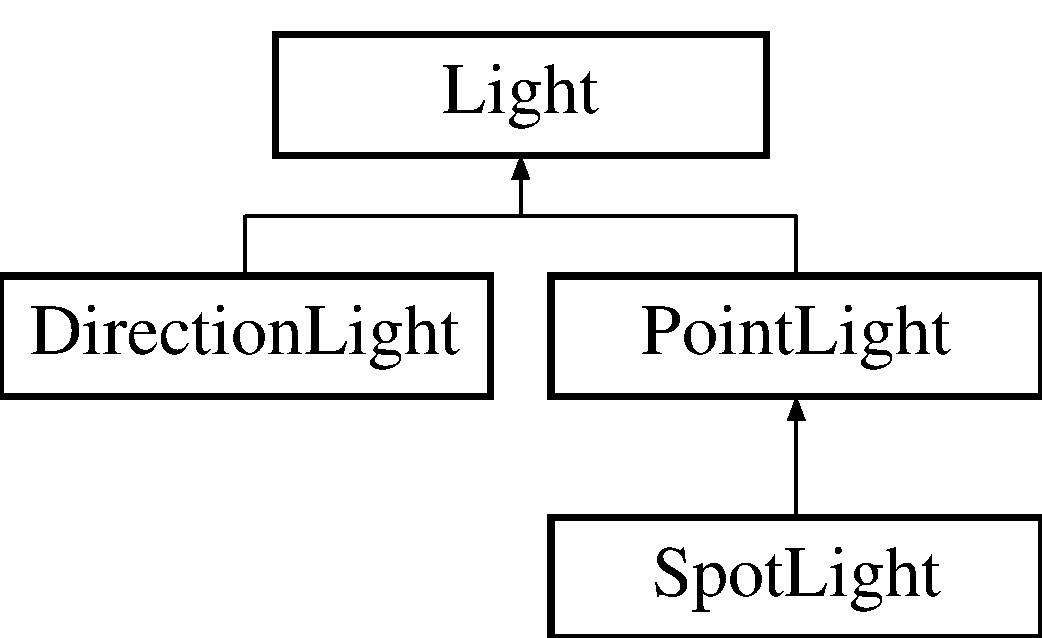
\includegraphics[height=3.000000cm]{classLight}
\end{center}
\end{figure}
\subsection*{Public Member Functions}
\begin{DoxyCompactItemize}
\item 
\hyperlink{classLight_aa563bb3ddf329e69f3026aafe309bb70}{Light} (const glm\+::vec3 \&pambient, const glm\+::vec3 \&pdiffuse, const glm\+::vec3 \&pspecular)
\item 
\hyperlink{classLight_aeb5df09a25a32f19fdffa761268ba24f}{Light} ()
\item 
virtual void \hyperlink{classLight_adfffa53d21bbeaa638c0bc5ae5a852cc}{set\+Uniforms} (const \hyperlink{classShader}{Shader} \&shader, const std\+::string \&uname) const
\item 
virtual void \hyperlink{classLight_a15770d3a4b173cd517477dfb5d5bcab9}{ui} ()
\end{DoxyCompactItemize}
\subsection*{Public Attributes}
\begin{DoxyCompactItemize}
\item 
glm\+::vec3 \hyperlink{classLight_ad255e60575bdb0ca5e9e63b738877327}{ambient\+\_\+}
\item 
glm\+::vec3 \hyperlink{classLight_ac5934c40340eb38365a9c090473c884f}{diffuse\+\_\+}
\item 
glm\+::vec3 \hyperlink{classLight_a9b425b4f0b04ec90da7de4bf77f30d1c}{specular\+\_\+}
\end{DoxyCompactItemize}


\subsection{Constructor \& Destructor Documentation}
\mbox{\Hypertarget{classLight_aa563bb3ddf329e69f3026aafe309bb70}\label{classLight_aa563bb3ddf329e69f3026aafe309bb70}} 
\index{Light@{Light}!Light@{Light}}
\index{Light@{Light}!Light@{Light}}
\subsubsection{\texorpdfstring{Light()}{Light()}\hspace{0.1cm}{\footnotesize\ttfamily [1/2]}}
{\footnotesize\ttfamily Light\+::\+Light (\begin{DoxyParamCaption}\item[{const glm\+::vec3 \&}]{pambient,  }\item[{const glm\+::vec3 \&}]{pdiffuse,  }\item[{const glm\+::vec3 \&}]{pspecular }\end{DoxyParamCaption})}

\mbox{\Hypertarget{classLight_aeb5df09a25a32f19fdffa761268ba24f}\label{classLight_aeb5df09a25a32f19fdffa761268ba24f}} 
\index{Light@{Light}!Light@{Light}}
\index{Light@{Light}!Light@{Light}}
\subsubsection{\texorpdfstring{Light()}{Light()}\hspace{0.1cm}{\footnotesize\ttfamily [2/2]}}
{\footnotesize\ttfamily Light\+::\+Light (\begin{DoxyParamCaption}{ }\end{DoxyParamCaption})}



\subsection{Member Function Documentation}
\mbox{\Hypertarget{classLight_adfffa53d21bbeaa638c0bc5ae5a852cc}\label{classLight_adfffa53d21bbeaa638c0bc5ae5a852cc}} 
\index{Light@{Light}!set\+Uniforms@{set\+Uniforms}}
\index{set\+Uniforms@{set\+Uniforms}!Light@{Light}}
\subsubsection{\texorpdfstring{set\+Uniforms()}{setUniforms()}}
{\footnotesize\ttfamily void Light\+::set\+Uniforms (\begin{DoxyParamCaption}\item[{const \hyperlink{classShader}{Shader} \&}]{shader,  }\item[{const std\+::string \&}]{uname }\end{DoxyParamCaption}) const\hspace{0.3cm}{\ttfamily [virtual]}}



Reimplemented in \hyperlink{classSpotLight_a4599dbd0a665514ff7066bfa01d04d1e}{Spot\+Light}, \hyperlink{classPointLight_abf6f298a0d04b636e22a3a5903e5b823}{Point\+Light}, and \hyperlink{classDirectionLight_ab10f7b680a8245bd4db3b7340593e485}{Direction\+Light}.

\mbox{\Hypertarget{classLight_a15770d3a4b173cd517477dfb5d5bcab9}\label{classLight_a15770d3a4b173cd517477dfb5d5bcab9}} 
\index{Light@{Light}!ui@{ui}}
\index{ui@{ui}!Light@{Light}}
\subsubsection{\texorpdfstring{ui()}{ui()}}
{\footnotesize\ttfamily void Light\+::ui (\begin{DoxyParamCaption}{ }\end{DoxyParamCaption})\hspace{0.3cm}{\ttfamily [virtual]}}



Reimplemented in \hyperlink{classSpotLight_a7ca46a2356ceb4f193704632e1f17bb4}{Spot\+Light}, \hyperlink{classPointLight_a538a42e0d1d713c57e46e492d352b34e}{Point\+Light}, and \hyperlink{classDirectionLight_a85ac86467a3053dea596b0ebf362b68f}{Direction\+Light}.



\subsection{Member Data Documentation}
\mbox{\Hypertarget{classLight_ad255e60575bdb0ca5e9e63b738877327}\label{classLight_ad255e60575bdb0ca5e9e63b738877327}} 
\index{Light@{Light}!ambient\+\_\+@{ambient\+\_\+}}
\index{ambient\+\_\+@{ambient\+\_\+}!Light@{Light}}
\subsubsection{\texorpdfstring{ambient\+\_\+}{ambient\_}}
{\footnotesize\ttfamily glm\+::vec3 Light\+::ambient\+\_\+}

\mbox{\Hypertarget{classLight_ac5934c40340eb38365a9c090473c884f}\label{classLight_ac5934c40340eb38365a9c090473c884f}} 
\index{Light@{Light}!diffuse\+\_\+@{diffuse\+\_\+}}
\index{diffuse\+\_\+@{diffuse\+\_\+}!Light@{Light}}
\subsubsection{\texorpdfstring{diffuse\+\_\+}{diffuse\_}}
{\footnotesize\ttfamily glm\+::vec3 Light\+::diffuse\+\_\+}

\mbox{\Hypertarget{classLight_a9b425b4f0b04ec90da7de4bf77f30d1c}\label{classLight_a9b425b4f0b04ec90da7de4bf77f30d1c}} 
\index{Light@{Light}!specular\+\_\+@{specular\+\_\+}}
\index{specular\+\_\+@{specular\+\_\+}!Light@{Light}}
\subsubsection{\texorpdfstring{specular\+\_\+}{specular\_}}
{\footnotesize\ttfamily glm\+::vec3 Light\+::specular\+\_\+}



The documentation for this class was generated from the following files\+:\begin{DoxyCompactItemize}
\item 
src/\hyperlink{light_8h}{light.\+h}\item 
src/\hyperlink{light_8cpp}{light.\+cpp}\end{DoxyCompactItemize}

\hypertarget{classMesh}{}\section{Mesh Class Reference}
\label{classMesh}\index{Mesh@{Mesh}}


\hyperlink{classMesh}{Mesh} wrapper.  




{\ttfamily \#include $<$mesh.\+h$>$}

\subsection*{Public Member Functions}
\begin{DoxyCompactItemize}
\item 
\hyperlink{classMesh_a54bd1b9e629ff006629579fc8fd6d002}{Mesh} (const std\+::vector$<$ \hyperlink{structVertex}{Vertex} $>$ \&vertices, const std\+::vector$<$ G\+Luint $>$ \&indices, const std\+::vector$<$ \hyperlink{structTexture}{Texture} $>$ \&textures)
\item 
void \hyperlink{classMesh_ab4a351fe96aa532b80232b2d7b0d55f2}{draw} (const \hyperlink{classShader}{Shader} \&shader, const G\+Lenum \&mode=-\/1) const
\begin{DoxyCompactList}\small\item\em Draw the model. \end{DoxyCompactList}\item 
void \hyperlink{classMesh_a66bf5cfb39cc2a96638769ad967be18a}{update\+Data\+Buffer} ()
\begin{DoxyCompactList}\small\item\em Update the data buffer. \end{DoxyCompactList}\end{DoxyCompactItemize}
\subsection*{Static Public Member Functions}
\begin{DoxyCompactItemize}
\item 
{\footnotesize template$<$class T $>$ }\\static void \hyperlink{classMesh_a5067620d30ba35b9f83e4dae7fb70cbf}{add\+Buffer} (G\+Luint \&id\+Location, G\+Lenum buf\+Type, const std\+::vector$<$ T $>$ \&data)
\begin{DoxyCompactList}\small\item\em Generate and allocate a buffer in the V\+AO. \end{DoxyCompactList}\end{DoxyCompactItemize}


\subsection{Detailed Description}
\hyperlink{classMesh}{Mesh} wrapper. 

Keep a link on the V\+B\+Os and V\+AO of a model. 

\subsection{Constructor \& Destructor Documentation}
\mbox{\Hypertarget{classMesh_a54bd1b9e629ff006629579fc8fd6d002}\label{classMesh_a54bd1b9e629ff006629579fc8fd6d002}} 
\index{Mesh@{Mesh}!Mesh@{Mesh}}
\index{Mesh@{Mesh}!Mesh@{Mesh}}
\subsubsection{\texorpdfstring{Mesh()}{Mesh()}}
{\footnotesize\ttfamily Mesh\+::\+Mesh (\begin{DoxyParamCaption}\item[{const std\+::vector$<$ \hyperlink{structVertex}{Vertex} $>$ \&}]{vertices,  }\item[{const std\+::vector$<$ G\+Luint $>$ \&}]{indices,  }\item[{const std\+::vector$<$ \hyperlink{structTexture}{Texture} $>$ \&}]{textures }\end{DoxyParamCaption})}



\subsection{Member Function Documentation}
\mbox{\Hypertarget{classMesh_a5067620d30ba35b9f83e4dae7fb70cbf}\label{classMesh_a5067620d30ba35b9f83e4dae7fb70cbf}} 
\index{Mesh@{Mesh}!add\+Buffer@{add\+Buffer}}
\index{add\+Buffer@{add\+Buffer}!Mesh@{Mesh}}
\subsubsection{\texorpdfstring{add\+Buffer()}{addBuffer()}}
{\footnotesize\ttfamily template$<$class T $>$ \\
void Mesh\+::add\+Buffer (\begin{DoxyParamCaption}\item[{G\+Luint \&}]{id\+Location,  }\item[{G\+Lenum}]{buf\+Type,  }\item[{const std\+::vector$<$ T $>$ \&}]{data }\end{DoxyParamCaption})\hspace{0.3cm}{\ttfamily [static]}}



Generate and allocate a buffer in the V\+AO. 


\begin{DoxyParams}{Parameters}
{\em id\+Location} & Where to store the id \\
\hline
{\em buf\+Type} & The buffer type \\
\hline
{\em data} & The points to copy in the buffer \\
\hline
\end{DoxyParams}
\mbox{\Hypertarget{classMesh_ab4a351fe96aa532b80232b2d7b0d55f2}\label{classMesh_ab4a351fe96aa532b80232b2d7b0d55f2}} 
\index{Mesh@{Mesh}!draw@{draw}}
\index{draw@{draw}!Mesh@{Mesh}}
\subsubsection{\texorpdfstring{draw()}{draw()}}
{\footnotesize\ttfamily void Mesh\+::draw (\begin{DoxyParamCaption}\item[{const \hyperlink{classShader}{Shader} \&}]{shader,  }\item[{const G\+Lenum \&}]{mode = {\ttfamily -\/1} }\end{DoxyParamCaption}) const}



Draw the model. 

\mbox{\Hypertarget{classMesh_a66bf5cfb39cc2a96638769ad967be18a}\label{classMesh_a66bf5cfb39cc2a96638769ad967be18a}} 
\index{Mesh@{Mesh}!update\+Data\+Buffer@{update\+Data\+Buffer}}
\index{update\+Data\+Buffer@{update\+Data\+Buffer}!Mesh@{Mesh}}
\subsubsection{\texorpdfstring{update\+Data\+Buffer()}{updateDataBuffer()}}
{\footnotesize\ttfamily void Mesh\+::update\+Data\+Buffer (\begin{DoxyParamCaption}{ }\end{DoxyParamCaption})}



Update the data buffer. 



The documentation for this class was generated from the following files\+:\begin{DoxyCompactItemize}
\item 
src/\hyperlink{mesh_8h}{mesh.\+h}\item 
src/\hyperlink{mesh_8cpp}{mesh.\+cpp}\end{DoxyCompactItemize}

\hypertarget{classModel}{}\section{Model Class Reference}
\label{classModel}\index{Model@{Model}}


A set of one or more mesh.  




{\ttfamily \#include $<$model.\+h$>$}

Inheritance diagram for Model\+:\begin{figure}[H]
\begin{center}
\leavevmode
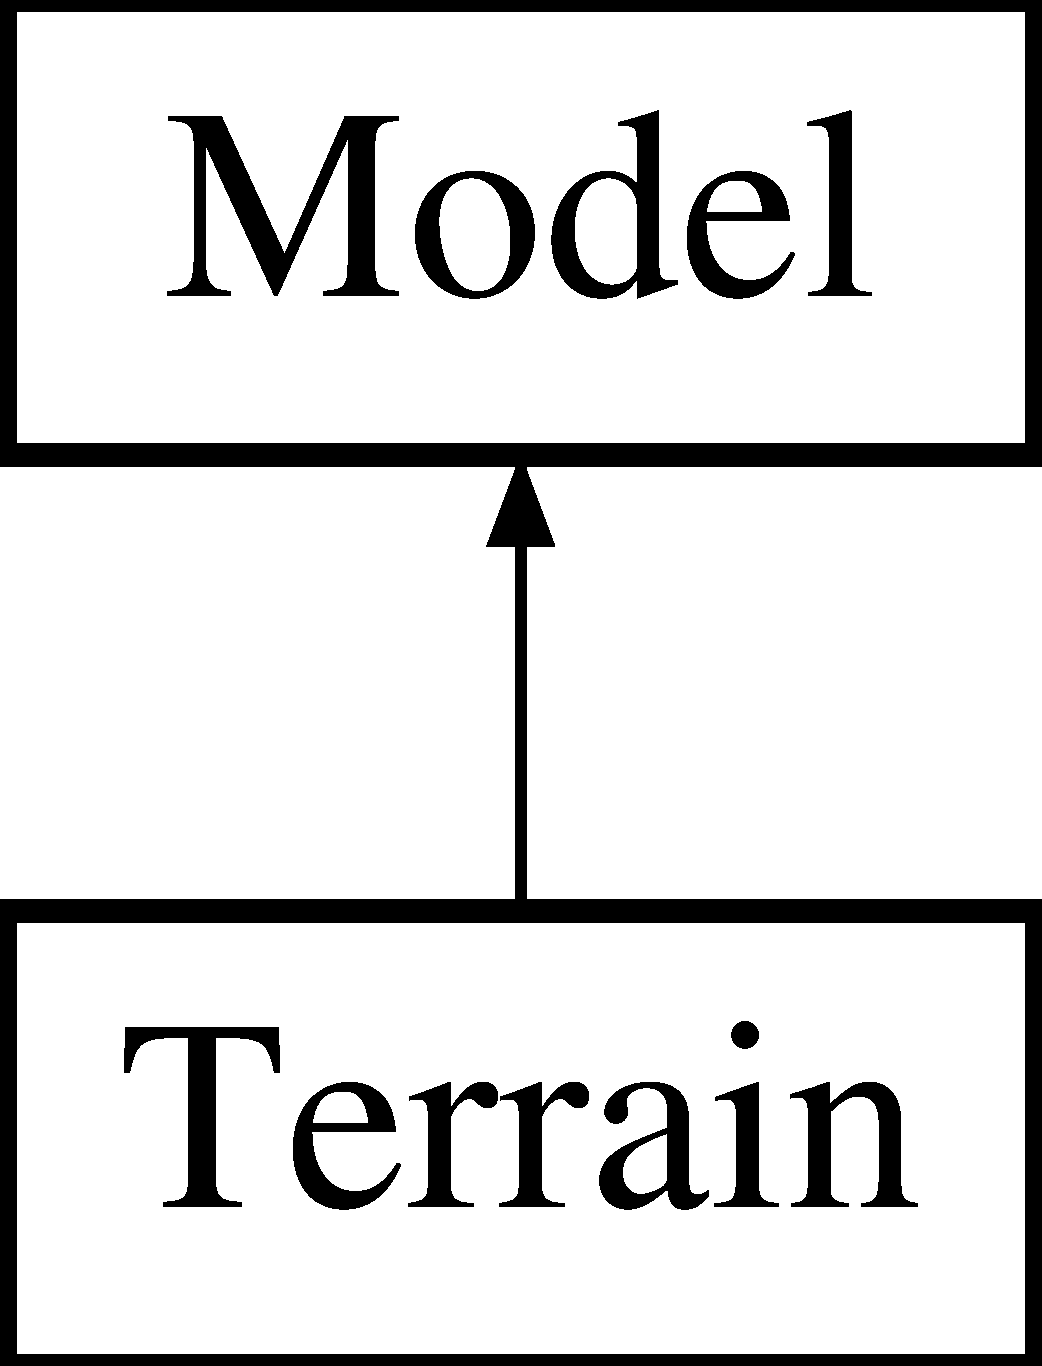
\includegraphics[height=2.000000cm]{classModel}
\end{center}
\end{figure}
\subsection*{Public Member Functions}
\begin{DoxyCompactItemize}
\item 
\hyperlink{classModel_ac455fa8d2babc9ea4d344d585a505ed5}{Model} (const std\+::string \&path)
\begin{DoxyCompactList}\small\item\em Create a model from a given path. \end{DoxyCompactList}\item 
virtual void \hyperlink{classModel_a125ff27c588f7f9acfc59c20dcc313b2}{draw} (const \hyperlink{classShader}{Shader} \&shader)
\begin{DoxyCompactList}\small\item\em Draw the model\textquotesingle{}s meshes. \end{DoxyCompactList}\item 
virtual void \hyperlink{classModel_a6c1d9003a9cb7699ba70b250c69d8ba4}{ui} ()
\end{DoxyCompactItemize}
\subsection*{Protected Member Functions}
\begin{DoxyCompactItemize}
\item 
\hyperlink{classModel_ae3b375de5f6df4faf74a95d64748e048}{Model} ()
\item 
void \hyperlink{classModel_a3d0a1ca0dc53b54cf5f6d956b156b7ec}{load\+Model} (const std\+::string \&path)
\begin{DoxyCompactList}\small\item\em Load the given model. \end{DoxyCompactList}\end{DoxyCompactItemize}
\subsection*{Protected Attributes}
\begin{DoxyCompactItemize}
\item 
std\+::vector$<$ \hyperlink{classMesh}{Mesh} $>$ \hyperlink{classModel_a538e42901dcfba59471072a48a162163}{meshes}
\begin{DoxyCompactList}\small\item\em Meshes included in the model. \end{DoxyCompactList}\end{DoxyCompactItemize}


\subsection{Detailed Description}
A set of one or more mesh. 

\subsection{Constructor \& Destructor Documentation}
\mbox{\Hypertarget{classModel_ac455fa8d2babc9ea4d344d585a505ed5}\label{classModel_ac455fa8d2babc9ea4d344d585a505ed5}} 
\index{Model@{Model}!Model@{Model}}
\index{Model@{Model}!Model@{Model}}
\subsubsection{\texorpdfstring{Model()}{Model()}\hspace{0.1cm}{\footnotesize\ttfamily [1/2]}}
{\footnotesize\ttfamily Model\+::\+Model (\begin{DoxyParamCaption}\item[{const std\+::string \&}]{path }\end{DoxyParamCaption})}



Create a model from a given path. 


\begin{DoxyParams}{Parameters}
{\em path} & Path to the object (obj) \\
\hline
\end{DoxyParams}
\mbox{\Hypertarget{classModel_ae3b375de5f6df4faf74a95d64748e048}\label{classModel_ae3b375de5f6df4faf74a95d64748e048}} 
\index{Model@{Model}!Model@{Model}}
\index{Model@{Model}!Model@{Model}}
\subsubsection{\texorpdfstring{Model()}{Model()}\hspace{0.1cm}{\footnotesize\ttfamily [2/2]}}
{\footnotesize\ttfamily Model\+::\+Model (\begin{DoxyParamCaption}{ }\end{DoxyParamCaption})\hspace{0.3cm}{\ttfamily [protected]}}



\subsection{Member Function Documentation}
\mbox{\Hypertarget{classModel_a125ff27c588f7f9acfc59c20dcc313b2}\label{classModel_a125ff27c588f7f9acfc59c20dcc313b2}} 
\index{Model@{Model}!draw@{draw}}
\index{draw@{draw}!Model@{Model}}
\subsubsection{\texorpdfstring{draw()}{draw()}}
{\footnotesize\ttfamily void Model\+::draw (\begin{DoxyParamCaption}\item[{const \hyperlink{classShader}{Shader} \&}]{shader }\end{DoxyParamCaption})\hspace{0.3cm}{\ttfamily [virtual]}}



Draw the model\textquotesingle{}s meshes. 


\begin{DoxyParams}{Parameters}
{\em shader} & \hyperlink{classShader}{Shader} used to draw \\
\hline
\end{DoxyParams}


Reimplemented in \hyperlink{classTerrain_ac3a615c383f37e7fc9894d20cc090da2}{Terrain}.

\mbox{\Hypertarget{classModel_a3d0a1ca0dc53b54cf5f6d956b156b7ec}\label{classModel_a3d0a1ca0dc53b54cf5f6d956b156b7ec}} 
\index{Model@{Model}!load\+Model@{load\+Model}}
\index{load\+Model@{load\+Model}!Model@{Model}}
\subsubsection{\texorpdfstring{load\+Model()}{loadModel()}}
{\footnotesize\ttfamily void Model\+::load\+Model (\begin{DoxyParamCaption}\item[{const std\+::string \&}]{path }\end{DoxyParamCaption})\hspace{0.3cm}{\ttfamily [protected]}}



Load the given model. 


\begin{DoxyParams}{Parameters}
{\em path} & Path to the model \\
\hline
\end{DoxyParams}
\mbox{\Hypertarget{classModel_a6c1d9003a9cb7699ba70b250c69d8ba4}\label{classModel_a6c1d9003a9cb7699ba70b250c69d8ba4}} 
\index{Model@{Model}!ui@{ui}}
\index{ui@{ui}!Model@{Model}}
\subsubsection{\texorpdfstring{ui()}{ui()}}
{\footnotesize\ttfamily void Model\+::ui (\begin{DoxyParamCaption}{ }\end{DoxyParamCaption})\hspace{0.3cm}{\ttfamily [virtual]}}



Reimplemented in \hyperlink{classTerrain_afff1911e27bd05cf1da59799db595322}{Terrain}.



\subsection{Member Data Documentation}
\mbox{\Hypertarget{classModel_a538e42901dcfba59471072a48a162163}\label{classModel_a538e42901dcfba59471072a48a162163}} 
\index{Model@{Model}!meshes@{meshes}}
\index{meshes@{meshes}!Model@{Model}}
\subsubsection{\texorpdfstring{meshes}{meshes}}
{\footnotesize\ttfamily std\+::vector$<$\hyperlink{classMesh}{Mesh}$>$ Model\+::meshes\hspace{0.3cm}{\ttfamily [protected]}}



Meshes included in the model. 



The documentation for this class was generated from the following files\+:\begin{DoxyCompactItemize}
\item 
src/\hyperlink{model_8h}{model.\+h}\item 
src/\hyperlink{model_8cpp}{model.\+cpp}\end{DoxyCompactItemize}

\hypertarget{classObject}{}\section{Object Class Reference}
\label{classObject}\index{Object@{Object}}


Wrapper of a model Can be positioned in the spaces Usefulle when creating instances, avoid to duplicate the model.  




{\ttfamily \#include $<$object.\+h$>$}

\subsection*{Public Member Functions}
\begin{DoxyCompactItemize}
\item 
\hyperlink{classObject_a40860402e64d8008fb42329df7097cdb}{Object} ()
\begin{DoxyCompactList}\small\item\em Create an empty object. Not used in the application yet. \end{DoxyCompactList}\item 
\hyperlink{classObject_a30ff0733f6b70bc1037d58b927237a0c}{Object} (std\+::shared\+\_\+ptr$<$ \hyperlink{classModel}{Model} $>$)
\begin{DoxyCompactList}\small\item\em Create a world object. \end{DoxyCompactList}\item 
void \hyperlink{classObject_ad9684af664b6b318174bb147d88131fe}{draw} (const \hyperlink{classShader}{Shader} \&shader)
\begin{DoxyCompactList}\small\item\em Draw the model\textquotesingle{}s meshes. \end{DoxyCompactList}\item 
void \hyperlink{classObject_a0a9d6c7d2325fc1eb7e5854151a51d09}{ui} ()
\item 
void \hyperlink{classObject_ac28acd7323fc00d2522b22b19a10a7d6}{random} ()
\begin{DoxyCompactList}\small\item\em change the object with new random (in range) parameters \end{DoxyCompactList}\end{DoxyCompactItemize}


\subsection{Detailed Description}
Wrapper of a model Can be positioned in the spaces Usefulle when creating instances, avoid to duplicate the model. 

\subsection{Constructor \& Destructor Documentation}
\mbox{\Hypertarget{classObject_a40860402e64d8008fb42329df7097cdb}\label{classObject_a40860402e64d8008fb42329df7097cdb}} 
\index{Object@{Object}!Object@{Object}}
\index{Object@{Object}!Object@{Object}}
\subsubsection{\texorpdfstring{Object()}{Object()}\hspace{0.1cm}{\footnotesize\ttfamily [1/2]}}
{\footnotesize\ttfamily Object\+::\+Object (\begin{DoxyParamCaption}{ }\end{DoxyParamCaption})}



Create an empty object. Not used in the application yet. 

\mbox{\Hypertarget{classObject_a30ff0733f6b70bc1037d58b927237a0c}\label{classObject_a30ff0733f6b70bc1037d58b927237a0c}} 
\index{Object@{Object}!Object@{Object}}
\index{Object@{Object}!Object@{Object}}
\subsubsection{\texorpdfstring{Object()}{Object()}\hspace{0.1cm}{\footnotesize\ttfamily [2/2]}}
{\footnotesize\ttfamily Object\+::\+Object (\begin{DoxyParamCaption}\item[{std\+::shared\+\_\+ptr$<$ \hyperlink{classModel}{Model} $>$}]{p\+Model }\end{DoxyParamCaption})}



Create a world object. 


\begin{DoxyParams}{Parameters}
{\em The} & model linked to the object \\
\hline
\end{DoxyParams}


\subsection{Member Function Documentation}
\mbox{\Hypertarget{classObject_ad9684af664b6b318174bb147d88131fe}\label{classObject_ad9684af664b6b318174bb147d88131fe}} 
\index{Object@{Object}!draw@{draw}}
\index{draw@{draw}!Object@{Object}}
\subsubsection{\texorpdfstring{draw()}{draw()}}
{\footnotesize\ttfamily void Object\+::draw (\begin{DoxyParamCaption}\item[{const \hyperlink{classShader}{Shader} \&}]{shader }\end{DoxyParamCaption})}



Draw the model\textquotesingle{}s meshes. 


\begin{DoxyParams}{Parameters}
{\em shader} & \hyperlink{classShader}{Shader} used to draw \\
\hline
\end{DoxyParams}
\mbox{\Hypertarget{classObject_ac28acd7323fc00d2522b22b19a10a7d6}\label{classObject_ac28acd7323fc00d2522b22b19a10a7d6}} 
\index{Object@{Object}!random@{random}}
\index{random@{random}!Object@{Object}}
\subsubsection{\texorpdfstring{random()}{random()}}
{\footnotesize\ttfamily void Object\+::random (\begin{DoxyParamCaption}{ }\end{DoxyParamCaption})}



change the object with new random (in range) parameters 

\mbox{\Hypertarget{classObject_a0a9d6c7d2325fc1eb7e5854151a51d09}\label{classObject_a0a9d6c7d2325fc1eb7e5854151a51d09}} 
\index{Object@{Object}!ui@{ui}}
\index{ui@{ui}!Object@{Object}}
\subsubsection{\texorpdfstring{ui()}{ui()}}
{\footnotesize\ttfamily void Object\+::ui (\begin{DoxyParamCaption}{ }\end{DoxyParamCaption})}



The documentation for this class was generated from the following files\+:\begin{DoxyCompactItemize}
\item 
src/\hyperlink{object_8h}{object.\+h}\item 
src/\hyperlink{object_8cpp}{object.\+cpp}\end{DoxyCompactItemize}

\hypertarget{classOrbitCamera}{}\section{Orbit\+Camera Class Reference}
\label{classOrbitCamera}\index{Orbit\+Camera@{Orbit\+Camera}}


\hyperlink{classCamera}{Camera} used to rotate around a round-\/shaped object.  




{\ttfamily \#include $<$orbit\+Camera.\+h$>$}

Inheritance diagram for Orbit\+Camera\+:\begin{figure}[H]
\begin{center}
\leavevmode
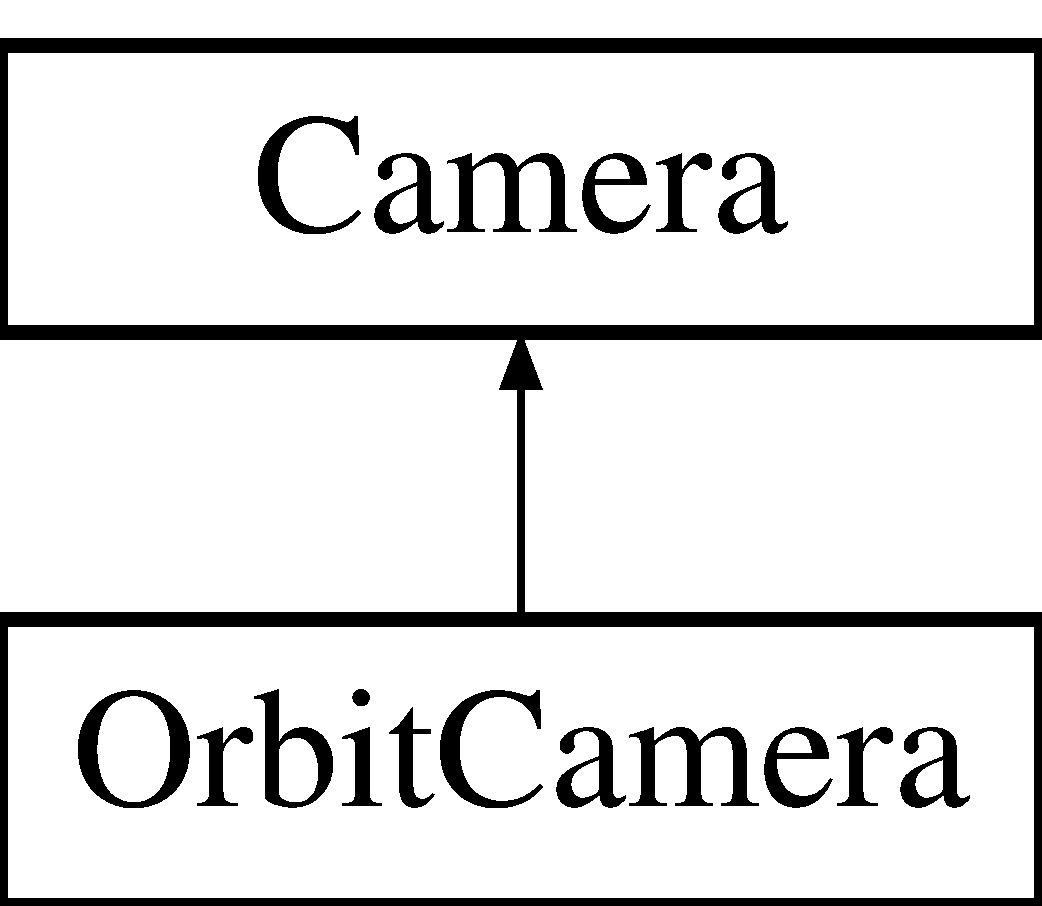
\includegraphics[height=2.000000cm]{classOrbitCamera}
\end{center}
\end{figure}
\subsection*{Public Member Functions}
\begin{DoxyCompactItemize}
\item 
\hyperlink{classOrbitCamera_ae87a8ab83042c47dac97a41ab4eb9e8c}{Orbit\+Camera} ()
\begin{DoxyCompactList}\small\item\em Create a camera with a default position and target. \end{DoxyCompactList}\item 
void \hyperlink{classOrbitCamera_a022751aa06693232844732adb00e7d71}{reset} ()
\begin{DoxyCompactList}\small\item\em Reset the camera target and position. \end{DoxyCompactList}\item 
void \hyperlink{classOrbitCamera_a73e280b9244dcbb6b8898a38d0243625}{process\+\_\+mouse\+\_\+move} (G\+L\+F\+Wwindow $\ast$window, double xpos, double ypos)
\item 
void \hyperlink{classOrbitCamera_af8cb999454725d091971106c4a7bf715}{process\+\_\+mouse\+\_\+action} (G\+L\+F\+Wwindow $\ast$window, int button, int action, int mods)
\item 
void \hyperlink{classOrbitCamera_a879faaab86c47e485e119d247279904f}{process\+\_\+scroll} (G\+L\+F\+Wwindow $\ast$window, double xoffset, double yoffset)
\item 
glm\+::mat4 \hyperlink{classOrbitCamera_a07595f9d11666c180934e47ba8abae73}{view} () const
\item 
glm\+::vec3 \hyperlink{classOrbitCamera_a1d65d137e3ef3f32c3b8eb31b49047fc}{up} () const
\end{DoxyCompactItemize}
\subsection*{Public Attributes}
\begin{DoxyCompactItemize}
\item 
glm\+::vec3 \hyperlink{classOrbitCamera_ab6f07eef6c4b0226b7abfc537b698c89}{target}
\end{DoxyCompactItemize}
\subsection*{Additional Inherited Members}


\subsection{Detailed Description}
\hyperlink{classCamera}{Camera} used to rotate around a round-\/shaped object. 

\subsection{Constructor \& Destructor Documentation}
\mbox{\Hypertarget{classOrbitCamera_ae87a8ab83042c47dac97a41ab4eb9e8c}\label{classOrbitCamera_ae87a8ab83042c47dac97a41ab4eb9e8c}} 
\index{Orbit\+Camera@{Orbit\+Camera}!Orbit\+Camera@{Orbit\+Camera}}
\index{Orbit\+Camera@{Orbit\+Camera}!Orbit\+Camera@{Orbit\+Camera}}
\subsubsection{\texorpdfstring{Orbit\+Camera()}{OrbitCamera()}}
{\footnotesize\ttfamily Orbit\+Camera\+::\+Orbit\+Camera (\begin{DoxyParamCaption}{ }\end{DoxyParamCaption})}



Create a camera with a default position and target. 



\subsection{Member Function Documentation}
\mbox{\Hypertarget{classOrbitCamera_af8cb999454725d091971106c4a7bf715}\label{classOrbitCamera_af8cb999454725d091971106c4a7bf715}} 
\index{Orbit\+Camera@{Orbit\+Camera}!process\+\_\+mouse\+\_\+action@{process\+\_\+mouse\+\_\+action}}
\index{process\+\_\+mouse\+\_\+action@{process\+\_\+mouse\+\_\+action}!Orbit\+Camera@{Orbit\+Camera}}
\subsubsection{\texorpdfstring{process\+\_\+mouse\+\_\+action()}{process\_mouse\_action()}}
{\footnotesize\ttfamily void Orbit\+Camera\+::process\+\_\+mouse\+\_\+action (\begin{DoxyParamCaption}\item[{G\+L\+F\+Wwindow $\ast$}]{window,  }\item[{int}]{button,  }\item[{int}]{action,  }\item[{int}]{mods }\end{DoxyParamCaption})\hspace{0.3cm}{\ttfamily [virtual]}}



Reimplemented from \hyperlink{classCamera_affd5e8a22d61e945ba56d2a807b98e61}{Camera}.

\mbox{\Hypertarget{classOrbitCamera_a73e280b9244dcbb6b8898a38d0243625}\label{classOrbitCamera_a73e280b9244dcbb6b8898a38d0243625}} 
\index{Orbit\+Camera@{Orbit\+Camera}!process\+\_\+mouse\+\_\+move@{process\+\_\+mouse\+\_\+move}}
\index{process\+\_\+mouse\+\_\+move@{process\+\_\+mouse\+\_\+move}!Orbit\+Camera@{Orbit\+Camera}}
\subsubsection{\texorpdfstring{process\+\_\+mouse\+\_\+move()}{process\_mouse\_move()}}
{\footnotesize\ttfamily void Orbit\+Camera\+::process\+\_\+mouse\+\_\+move (\begin{DoxyParamCaption}\item[{G\+L\+F\+Wwindow $\ast$}]{window,  }\item[{double}]{xpos,  }\item[{double}]{ypos }\end{DoxyParamCaption})\hspace{0.3cm}{\ttfamily [virtual]}}



Reimplemented from \hyperlink{classCamera_abb67395d3094b766d86ad17cedc054c3}{Camera}.

\mbox{\Hypertarget{classOrbitCamera_a879faaab86c47e485e119d247279904f}\label{classOrbitCamera_a879faaab86c47e485e119d247279904f}} 
\index{Orbit\+Camera@{Orbit\+Camera}!process\+\_\+scroll@{process\+\_\+scroll}}
\index{process\+\_\+scroll@{process\+\_\+scroll}!Orbit\+Camera@{Orbit\+Camera}}
\subsubsection{\texorpdfstring{process\+\_\+scroll()}{process\_scroll()}}
{\footnotesize\ttfamily void Orbit\+Camera\+::process\+\_\+scroll (\begin{DoxyParamCaption}\item[{G\+L\+F\+Wwindow $\ast$}]{window,  }\item[{double}]{xoffset,  }\item[{double}]{yoffset }\end{DoxyParamCaption})\hspace{0.3cm}{\ttfamily [virtual]}}



Reimplemented from \hyperlink{classCamera_ac13cc5fa7a3a5c40e53d95e987c1ff04}{Camera}.

\mbox{\Hypertarget{classOrbitCamera_a022751aa06693232844732adb00e7d71}\label{classOrbitCamera_a022751aa06693232844732adb00e7d71}} 
\index{Orbit\+Camera@{Orbit\+Camera}!reset@{reset}}
\index{reset@{reset}!Orbit\+Camera@{Orbit\+Camera}}
\subsubsection{\texorpdfstring{reset()}{reset()}}
{\footnotesize\ttfamily void Orbit\+Camera\+::reset (\begin{DoxyParamCaption}{ }\end{DoxyParamCaption})\hspace{0.3cm}{\ttfamily [virtual]}}



Reset the camera target and position. 



Implements \hyperlink{classCamera_aa7695a960438e5571e14f50ed69f6623}{Camera}.

\mbox{\Hypertarget{classOrbitCamera_a1d65d137e3ef3f32c3b8eb31b49047fc}\label{classOrbitCamera_a1d65d137e3ef3f32c3b8eb31b49047fc}} 
\index{Orbit\+Camera@{Orbit\+Camera}!up@{up}}
\index{up@{up}!Orbit\+Camera@{Orbit\+Camera}}
\subsubsection{\texorpdfstring{up()}{up()}}
{\footnotesize\ttfamily glm\+::vec3 Orbit\+Camera\+::up (\begin{DoxyParamCaption}{ }\end{DoxyParamCaption}) const\hspace{0.3cm}{\ttfamily [virtual]}}



Implements \hyperlink{classCamera_a3ec282533cfc02be93006259d383b6d2}{Camera}.

\mbox{\Hypertarget{classOrbitCamera_a07595f9d11666c180934e47ba8abae73}\label{classOrbitCamera_a07595f9d11666c180934e47ba8abae73}} 
\index{Orbit\+Camera@{Orbit\+Camera}!view@{view}}
\index{view@{view}!Orbit\+Camera@{Orbit\+Camera}}
\subsubsection{\texorpdfstring{view()}{view()}}
{\footnotesize\ttfamily glm\+::mat4 Orbit\+Camera\+::view (\begin{DoxyParamCaption}{ }\end{DoxyParamCaption}) const\hspace{0.3cm}{\ttfamily [virtual]}}



Implements \hyperlink{classCamera_a279a5a9fdcdb6161bab2c3ff8fce275b}{Camera}.



\subsection{Member Data Documentation}
\mbox{\Hypertarget{classOrbitCamera_ab6f07eef6c4b0226b7abfc537b698c89}\label{classOrbitCamera_ab6f07eef6c4b0226b7abfc537b698c89}} 
\index{Orbit\+Camera@{Orbit\+Camera}!target@{target}}
\index{target@{target}!Orbit\+Camera@{Orbit\+Camera}}
\subsubsection{\texorpdfstring{target}{target}}
{\footnotesize\ttfamily glm\+::vec3 Orbit\+Camera\+::target}



The documentation for this class was generated from the following files\+:\begin{DoxyCompactItemize}
\item 
src/\hyperlink{orbitCamera_8h}{orbit\+Camera.\+h}\item 
src/\hyperlink{orbitCamera_8cpp}{orbit\+Camera.\+cpp}\end{DoxyCompactItemize}

\hypertarget{classPointLight}{}\section{Point\+Light Class Reference}
\label{classPointLight}\index{Point\+Light@{Point\+Light}}


{\ttfamily \#include $<$light.\+h$>$}

Inheritance diagram for Point\+Light\+:\begin{figure}[H]
\begin{center}
\leavevmode
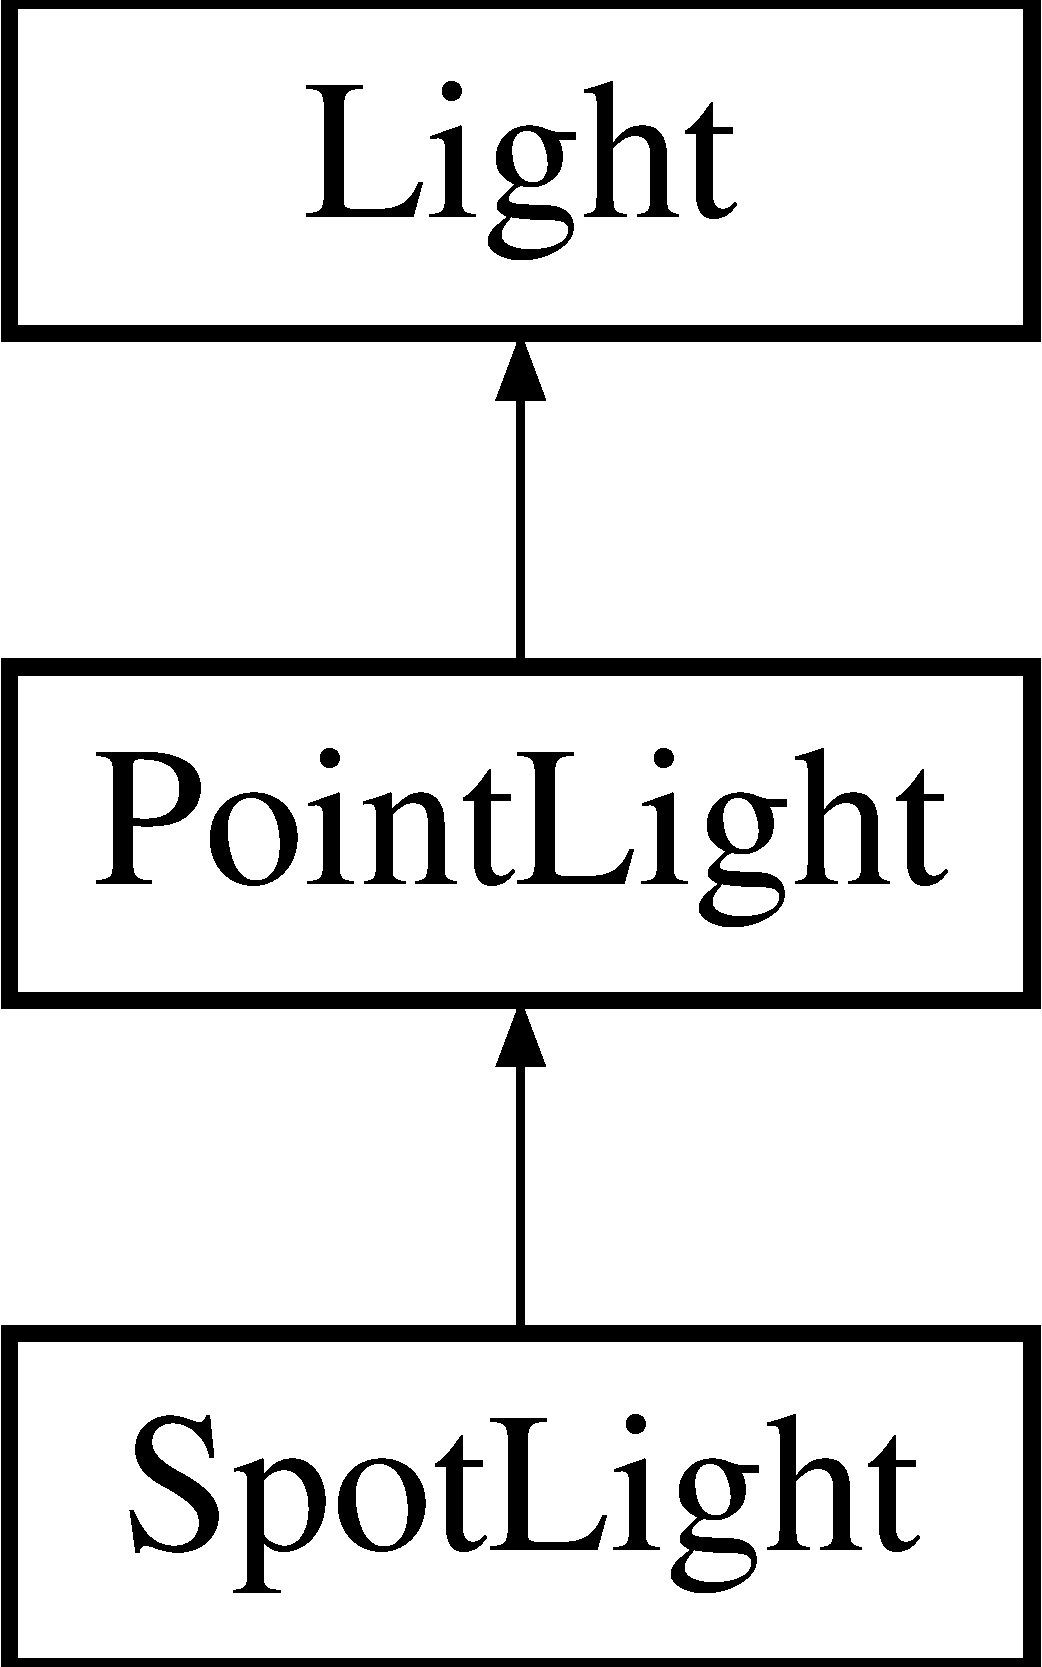
\includegraphics[height=3.000000cm]{classPointLight}
\end{center}
\end{figure}
\subsection*{Public Member Functions}
\begin{DoxyCompactItemize}
\item 
virtual void \hyperlink{classPointLight_abf6f298a0d04b636e22a3a5903e5b823}{set\+Uniforms} (const \hyperlink{classShader}{Shader} \&shader, const std\+::string \&uname) const
\item 
virtual void \hyperlink{classPointLight_a538a42e0d1d713c57e46e492d352b34e}{ui} ()
\end{DoxyCompactItemize}
\subsection*{Public Attributes}
\begin{DoxyCompactItemize}
\item 
glm\+::vec3 \hyperlink{classPointLight_a6ab3a936be50472a3b5a064edc18f5ce}{position\+\_\+} = \{5.f, 5.f, 5.f\}
\item 
float \hyperlink{classPointLight_ac66b99d54650b57401ae4f7d3c1c22f4}{constant\+\_\+} = 1
\item 
float \hyperlink{classPointLight_a11a41268a4d9e19d45eed18ba1ad8e43}{linear\+\_\+} = 0.\+09
\item 
float \hyperlink{classPointLight_a7adf3997d566c55fb2878db179d4867d}{quadratic\+\_\+} = 0.\+032
\end{DoxyCompactItemize}


\subsection{Member Function Documentation}
\mbox{\Hypertarget{classPointLight_abf6f298a0d04b636e22a3a5903e5b823}\label{classPointLight_abf6f298a0d04b636e22a3a5903e5b823}} 
\index{Point\+Light@{Point\+Light}!set\+Uniforms@{set\+Uniforms}}
\index{set\+Uniforms@{set\+Uniforms}!Point\+Light@{Point\+Light}}
\subsubsection{\texorpdfstring{set\+Uniforms()}{setUniforms()}}
{\footnotesize\ttfamily void Point\+Light\+::set\+Uniforms (\begin{DoxyParamCaption}\item[{const \hyperlink{classShader}{Shader} \&}]{shader,  }\item[{const std\+::string \&}]{uname }\end{DoxyParamCaption}) const\hspace{0.3cm}{\ttfamily [virtual]}}



Reimplemented from \hyperlink{classLight_adfffa53d21bbeaa638c0bc5ae5a852cc}{Light}.



Reimplemented in \hyperlink{classSpotLight_a4599dbd0a665514ff7066bfa01d04d1e}{Spot\+Light}.

\mbox{\Hypertarget{classPointLight_a538a42e0d1d713c57e46e492d352b34e}\label{classPointLight_a538a42e0d1d713c57e46e492d352b34e}} 
\index{Point\+Light@{Point\+Light}!ui@{ui}}
\index{ui@{ui}!Point\+Light@{Point\+Light}}
\subsubsection{\texorpdfstring{ui()}{ui()}}
{\footnotesize\ttfamily void Point\+Light\+::ui (\begin{DoxyParamCaption}{ }\end{DoxyParamCaption})\hspace{0.3cm}{\ttfamily [virtual]}}



Reimplemented from \hyperlink{classLight_a15770d3a4b173cd517477dfb5d5bcab9}{Light}.



Reimplemented in \hyperlink{classSpotLight_a7ca46a2356ceb4f193704632e1f17bb4}{Spot\+Light}.



\subsection{Member Data Documentation}
\mbox{\Hypertarget{classPointLight_ac66b99d54650b57401ae4f7d3c1c22f4}\label{classPointLight_ac66b99d54650b57401ae4f7d3c1c22f4}} 
\index{Point\+Light@{Point\+Light}!constant\+\_\+@{constant\+\_\+}}
\index{constant\+\_\+@{constant\+\_\+}!Point\+Light@{Point\+Light}}
\subsubsection{\texorpdfstring{constant\+\_\+}{constant\_}}
{\footnotesize\ttfamily float Point\+Light\+::constant\+\_\+ = 1}

\mbox{\Hypertarget{classPointLight_a11a41268a4d9e19d45eed18ba1ad8e43}\label{classPointLight_a11a41268a4d9e19d45eed18ba1ad8e43}} 
\index{Point\+Light@{Point\+Light}!linear\+\_\+@{linear\+\_\+}}
\index{linear\+\_\+@{linear\+\_\+}!Point\+Light@{Point\+Light}}
\subsubsection{\texorpdfstring{linear\+\_\+}{linear\_}}
{\footnotesize\ttfamily float Point\+Light\+::linear\+\_\+ = 0.\+09}

\mbox{\Hypertarget{classPointLight_a6ab3a936be50472a3b5a064edc18f5ce}\label{classPointLight_a6ab3a936be50472a3b5a064edc18f5ce}} 
\index{Point\+Light@{Point\+Light}!position\+\_\+@{position\+\_\+}}
\index{position\+\_\+@{position\+\_\+}!Point\+Light@{Point\+Light}}
\subsubsection{\texorpdfstring{position\+\_\+}{position\_}}
{\footnotesize\ttfamily glm\+::vec3 Point\+Light\+::position\+\_\+ = \{5.f, 5.f, 5.f\}}

\mbox{\Hypertarget{classPointLight_a7adf3997d566c55fb2878db179d4867d}\label{classPointLight_a7adf3997d566c55fb2878db179d4867d}} 
\index{Point\+Light@{Point\+Light}!quadratic\+\_\+@{quadratic\+\_\+}}
\index{quadratic\+\_\+@{quadratic\+\_\+}!Point\+Light@{Point\+Light}}
\subsubsection{\texorpdfstring{quadratic\+\_\+}{quadratic\_}}
{\footnotesize\ttfamily float Point\+Light\+::quadratic\+\_\+ = 0.\+032}



The documentation for this class was generated from the following files\+:\begin{DoxyCompactItemize}
\item 
src/\hyperlink{light_8h}{light.\+h}\item 
src/\hyperlink{light_8cpp}{light.\+cpp}\end{DoxyCompactItemize}

\hypertarget{classShader}{}\section{Shader Class Reference}
\label{classShader}\index{Shader@{Shader}}


{\ttfamily \#include $<$shader.\+h$>$}

\subsection*{Public Member Functions}
\begin{DoxyCompactItemize}
\item 
\hyperlink{classShader_a7e347bafb56502a85791603d3e52ba3c}{Shader} (const std\+::string \&vert\+Src\+Path, const std\+::string \&frag\+Src\+Path, const std\+::string \&geo\+Src\+Path=\char`\"{}\char`\"{})
\begin{DoxyCompactList}\small\item\em Create and compile a shader. \end{DoxyCompactList}\item 
\hyperlink{classShader_af43c2f34d90b61fd66c3b365f42392b2}{Shader} (std\+::string path, const bool \&use\+Geo=false)
\begin{DoxyCompactList}\small\item\em Create and compile a shader with sources using same name but different extension. \end{DoxyCompactList}\item 
void \hyperlink{classShader_a3c7896754f0e1fca8bde860cfef63832}{use} () const
\begin{DoxyCompactList}\small\item\em Use the shader with gl\+Use\+Program. \end{DoxyCompactList}\item 
void \hyperlink{classShader_ab1a56d6c299bd7eaa18c2e142ef7bd9f}{set\+Bool} (const std\+::string \&name, bool value) const
\item 
void \hyperlink{classShader_ad362e2b654cd95a3574cd505411e41fd}{set\+Int} (const std\+::string \&name, int value) const
\item 
void \hyperlink{classShader_afe7367621f74c2d26431d8ac15252bf3}{set\+Float} (const std\+::string \&name, float value) const
\item 
void \hyperlink{classShader_afd4d41322a1cdd1d5155bf124d19debf}{set\+Vec2} (const std\+::string \&name, const glm\+::vec2 \&value) const
\item 
void \hyperlink{classShader_afb91bc9e954bf590857c96ab1331b0ec}{set\+Vec2} (const std\+::string \&name, float x, float y) const
\item 
void \hyperlink{classShader_aeb021061c5d451329d92257b07dbfec3}{set\+Vec3} (const std\+::string \&name, const glm\+::vec3 \&value) const
\item 
void \hyperlink{classShader_a90092c25b7dc23964c465b93887300f9}{set\+Vec3} (const std\+::string \&name, float x, float y, float z) const
\item 
void \hyperlink{classShader_a79cbe674f6bf1a576a48045dcb924de5}{set\+Vec4} (const std\+::string \&name, const glm\+::vec4 \&value) const
\item 
void \hyperlink{classShader_a913e10fe2501b00746ae6901b97a1730}{set\+Vec4} (const std\+::string \&name, float x, float y, float z, float w)
\item 
void \hyperlink{classShader_a91a6ee79b959cacd618c9e29a5bbd732}{set\+Mat2} (const std\+::string \&name, const glm\+::mat2 \&mat) const
\item 
void \hyperlink{classShader_a3e24fcad187493dfebaa12939072e91d}{set\+Mat3} (const std\+::string \&name, const glm\+::mat3 \&mat) const
\item 
void \hyperlink{classShader_a8e711c96f3e1722cbfb88fde9478977c}{set\+Mat4} (const std\+::string \&name, const glm\+::mat4 \&mat) const
\end{DoxyCompactItemize}


\subsection{Constructor \& Destructor Documentation}
\mbox{\Hypertarget{classShader_a7e347bafb56502a85791603d3e52ba3c}\label{classShader_a7e347bafb56502a85791603d3e52ba3c}} 
\index{Shader@{Shader}!Shader@{Shader}}
\index{Shader@{Shader}!Shader@{Shader}}
\subsubsection{\texorpdfstring{Shader()}{Shader()}\hspace{0.1cm}{\footnotesize\ttfamily [1/2]}}
{\footnotesize\ttfamily Shader\+::\+Shader (\begin{DoxyParamCaption}\item[{const std\+::string \&}]{vert\+Src\+Path,  }\item[{const std\+::string \&}]{frag\+Src\+Path,  }\item[{const std\+::string \&}]{geo\+Src\+Path = {\ttfamily \char`\"{}\char`\"{}} }\end{DoxyParamCaption})}



Create and compile a shader. 


\begin{DoxyParams}{Parameters}
{\em vert\+Src\+Path} & Path to the vertex shader source \\
\hline
{\em frag\+Src\+Path} & Path to the fragment shader soruce \\
\hline
{\em geo\+Src\+Path} & Path to the geometry shader source (default=null) \\
\hline
\end{DoxyParams}
\mbox{\Hypertarget{classShader_af43c2f34d90b61fd66c3b365f42392b2}\label{classShader_af43c2f34d90b61fd66c3b365f42392b2}} 
\index{Shader@{Shader}!Shader@{Shader}}
\index{Shader@{Shader}!Shader@{Shader}}
\subsubsection{\texorpdfstring{Shader()}{Shader()}\hspace{0.1cm}{\footnotesize\ttfamily [2/2]}}
{\footnotesize\ttfamily Shader\+::\+Shader (\begin{DoxyParamCaption}\item[{std\+::string}]{path,  }\item[{const bool \&}]{use\+Geo = {\ttfamily false} }\end{DoxyParamCaption})\hspace{0.3cm}{\ttfamily [explicit]}}



Create and compile a shader with sources using same name but different extension. 


\begin{DoxyParams}{Parameters}
{\em path} & Path to the source without extension \\
\hline
{\em use\+Geo} & If true, use the geo shader \\
\hline
\end{DoxyParams}


\subsection{Member Function Documentation}
\mbox{\Hypertarget{classShader_ab1a56d6c299bd7eaa18c2e142ef7bd9f}\label{classShader_ab1a56d6c299bd7eaa18c2e142ef7bd9f}} 
\index{Shader@{Shader}!set\+Bool@{set\+Bool}}
\index{set\+Bool@{set\+Bool}!Shader@{Shader}}
\subsubsection{\texorpdfstring{set\+Bool()}{setBool()}}
{\footnotesize\ttfamily void Shader\+::set\+Bool (\begin{DoxyParamCaption}\item[{const std\+::string \&}]{name,  }\item[{bool}]{value }\end{DoxyParamCaption}) const\hspace{0.3cm}{\ttfamily [inline]}}

\mbox{\Hypertarget{classShader_afe7367621f74c2d26431d8ac15252bf3}\label{classShader_afe7367621f74c2d26431d8ac15252bf3}} 
\index{Shader@{Shader}!set\+Float@{set\+Float}}
\index{set\+Float@{set\+Float}!Shader@{Shader}}
\subsubsection{\texorpdfstring{set\+Float()}{setFloat()}}
{\footnotesize\ttfamily void Shader\+::set\+Float (\begin{DoxyParamCaption}\item[{const std\+::string \&}]{name,  }\item[{float}]{value }\end{DoxyParamCaption}) const\hspace{0.3cm}{\ttfamily [inline]}}

\mbox{\Hypertarget{classShader_ad362e2b654cd95a3574cd505411e41fd}\label{classShader_ad362e2b654cd95a3574cd505411e41fd}} 
\index{Shader@{Shader}!set\+Int@{set\+Int}}
\index{set\+Int@{set\+Int}!Shader@{Shader}}
\subsubsection{\texorpdfstring{set\+Int()}{setInt()}}
{\footnotesize\ttfamily void Shader\+::set\+Int (\begin{DoxyParamCaption}\item[{const std\+::string \&}]{name,  }\item[{int}]{value }\end{DoxyParamCaption}) const\hspace{0.3cm}{\ttfamily [inline]}}

\mbox{\Hypertarget{classShader_a91a6ee79b959cacd618c9e29a5bbd732}\label{classShader_a91a6ee79b959cacd618c9e29a5bbd732}} 
\index{Shader@{Shader}!set\+Mat2@{set\+Mat2}}
\index{set\+Mat2@{set\+Mat2}!Shader@{Shader}}
\subsubsection{\texorpdfstring{set\+Mat2()}{setMat2()}}
{\footnotesize\ttfamily void Shader\+::set\+Mat2 (\begin{DoxyParamCaption}\item[{const std\+::string \&}]{name,  }\item[{const glm\+::mat2 \&}]{mat }\end{DoxyParamCaption}) const\hspace{0.3cm}{\ttfamily [inline]}}

\mbox{\Hypertarget{classShader_a3e24fcad187493dfebaa12939072e91d}\label{classShader_a3e24fcad187493dfebaa12939072e91d}} 
\index{Shader@{Shader}!set\+Mat3@{set\+Mat3}}
\index{set\+Mat3@{set\+Mat3}!Shader@{Shader}}
\subsubsection{\texorpdfstring{set\+Mat3()}{setMat3()}}
{\footnotesize\ttfamily void Shader\+::set\+Mat3 (\begin{DoxyParamCaption}\item[{const std\+::string \&}]{name,  }\item[{const glm\+::mat3 \&}]{mat }\end{DoxyParamCaption}) const\hspace{0.3cm}{\ttfamily [inline]}}

\mbox{\Hypertarget{classShader_a8e711c96f3e1722cbfb88fde9478977c}\label{classShader_a8e711c96f3e1722cbfb88fde9478977c}} 
\index{Shader@{Shader}!set\+Mat4@{set\+Mat4}}
\index{set\+Mat4@{set\+Mat4}!Shader@{Shader}}
\subsubsection{\texorpdfstring{set\+Mat4()}{setMat4()}}
{\footnotesize\ttfamily void Shader\+::set\+Mat4 (\begin{DoxyParamCaption}\item[{const std\+::string \&}]{name,  }\item[{const glm\+::mat4 \&}]{mat }\end{DoxyParamCaption}) const\hspace{0.3cm}{\ttfamily [inline]}}

\mbox{\Hypertarget{classShader_afd4d41322a1cdd1d5155bf124d19debf}\label{classShader_afd4d41322a1cdd1d5155bf124d19debf}} 
\index{Shader@{Shader}!set\+Vec2@{set\+Vec2}}
\index{set\+Vec2@{set\+Vec2}!Shader@{Shader}}
\subsubsection{\texorpdfstring{set\+Vec2()}{setVec2()}\hspace{0.1cm}{\footnotesize\ttfamily [1/2]}}
{\footnotesize\ttfamily void Shader\+::set\+Vec2 (\begin{DoxyParamCaption}\item[{const std\+::string \&}]{name,  }\item[{const glm\+::vec2 \&}]{value }\end{DoxyParamCaption}) const\hspace{0.3cm}{\ttfamily [inline]}}

\mbox{\Hypertarget{classShader_afb91bc9e954bf590857c96ab1331b0ec}\label{classShader_afb91bc9e954bf590857c96ab1331b0ec}} 
\index{Shader@{Shader}!set\+Vec2@{set\+Vec2}}
\index{set\+Vec2@{set\+Vec2}!Shader@{Shader}}
\subsubsection{\texorpdfstring{set\+Vec2()}{setVec2()}\hspace{0.1cm}{\footnotesize\ttfamily [2/2]}}
{\footnotesize\ttfamily void Shader\+::set\+Vec2 (\begin{DoxyParamCaption}\item[{const std\+::string \&}]{name,  }\item[{float}]{x,  }\item[{float}]{y }\end{DoxyParamCaption}) const\hspace{0.3cm}{\ttfamily [inline]}}

\mbox{\Hypertarget{classShader_aeb021061c5d451329d92257b07dbfec3}\label{classShader_aeb021061c5d451329d92257b07dbfec3}} 
\index{Shader@{Shader}!set\+Vec3@{set\+Vec3}}
\index{set\+Vec3@{set\+Vec3}!Shader@{Shader}}
\subsubsection{\texorpdfstring{set\+Vec3()}{setVec3()}\hspace{0.1cm}{\footnotesize\ttfamily [1/2]}}
{\footnotesize\ttfamily void Shader\+::set\+Vec3 (\begin{DoxyParamCaption}\item[{const std\+::string \&}]{name,  }\item[{const glm\+::vec3 \&}]{value }\end{DoxyParamCaption}) const\hspace{0.3cm}{\ttfamily [inline]}}

\mbox{\Hypertarget{classShader_a90092c25b7dc23964c465b93887300f9}\label{classShader_a90092c25b7dc23964c465b93887300f9}} 
\index{Shader@{Shader}!set\+Vec3@{set\+Vec3}}
\index{set\+Vec3@{set\+Vec3}!Shader@{Shader}}
\subsubsection{\texorpdfstring{set\+Vec3()}{setVec3()}\hspace{0.1cm}{\footnotesize\ttfamily [2/2]}}
{\footnotesize\ttfamily void Shader\+::set\+Vec3 (\begin{DoxyParamCaption}\item[{const std\+::string \&}]{name,  }\item[{float}]{x,  }\item[{float}]{y,  }\item[{float}]{z }\end{DoxyParamCaption}) const\hspace{0.3cm}{\ttfamily [inline]}}

\mbox{\Hypertarget{classShader_a79cbe674f6bf1a576a48045dcb924de5}\label{classShader_a79cbe674f6bf1a576a48045dcb924de5}} 
\index{Shader@{Shader}!set\+Vec4@{set\+Vec4}}
\index{set\+Vec4@{set\+Vec4}!Shader@{Shader}}
\subsubsection{\texorpdfstring{set\+Vec4()}{setVec4()}\hspace{0.1cm}{\footnotesize\ttfamily [1/2]}}
{\footnotesize\ttfamily void Shader\+::set\+Vec4 (\begin{DoxyParamCaption}\item[{const std\+::string \&}]{name,  }\item[{const glm\+::vec4 \&}]{value }\end{DoxyParamCaption}) const\hspace{0.3cm}{\ttfamily [inline]}}

\mbox{\Hypertarget{classShader_a913e10fe2501b00746ae6901b97a1730}\label{classShader_a913e10fe2501b00746ae6901b97a1730}} 
\index{Shader@{Shader}!set\+Vec4@{set\+Vec4}}
\index{set\+Vec4@{set\+Vec4}!Shader@{Shader}}
\subsubsection{\texorpdfstring{set\+Vec4()}{setVec4()}\hspace{0.1cm}{\footnotesize\ttfamily [2/2]}}
{\footnotesize\ttfamily void Shader\+::set\+Vec4 (\begin{DoxyParamCaption}\item[{const std\+::string \&}]{name,  }\item[{float}]{x,  }\item[{float}]{y,  }\item[{float}]{z,  }\item[{float}]{w }\end{DoxyParamCaption})\hspace{0.3cm}{\ttfamily [inline]}}

\mbox{\Hypertarget{classShader_a3c7896754f0e1fca8bde860cfef63832}\label{classShader_a3c7896754f0e1fca8bde860cfef63832}} 
\index{Shader@{Shader}!use@{use}}
\index{use@{use}!Shader@{Shader}}
\subsubsection{\texorpdfstring{use()}{use()}}
{\footnotesize\ttfamily void Shader\+::use (\begin{DoxyParamCaption}{ }\end{DoxyParamCaption}) const}



Use the shader with gl\+Use\+Program. 



The documentation for this class was generated from the following files\+:\begin{DoxyCompactItemize}
\item 
src/\hyperlink{shader_8h}{shader.\+h}\item 
src/\hyperlink{shader_8cpp}{shader.\+cpp}\end{DoxyCompactItemize}

\hypertarget{classSkyBox}{}\section{Sky\+Box Class Reference}
\label{classSkyBox}\index{Sky\+Box@{Sky\+Box}}


A Cubemap.  




{\ttfamily \#include $<$skybox.\+h$>$}

\subsection*{Public Member Functions}
\begin{DoxyCompactItemize}
\item 
\hyperlink{classSkyBox_ad707af7cdeec0647cebcfb46698790d9}{Sky\+Box} (const std\+::string \&, const std\+::string \&)
\begin{DoxyCompactList}\small\item\em Create a skybox by specifying the file path and the extension ex\+: world, .png, will use world\+\_\+bk.\+png, ... \end{DoxyCompactList}\item 
void \hyperlink{classSkyBox_a366982874c361360c654015e794b1e22}{draw} (\hyperlink{classShader}{Shader} \&sh)
\begin{DoxyCompactList}\small\item\em Draw the Skybox. \end{DoxyCompactList}\end{DoxyCompactItemize}
\subsection*{Protected Attributes}
\begin{DoxyCompactItemize}
\item 
G\+Luint \hyperlink{classSkyBox_af762eed644f128a560e22d5003c5d447}{vao}
\item 
G\+Luint \hyperlink{classSkyBox_ad62d8584917884e9f154421ea637888b}{cubemap}
\end{DoxyCompactItemize}


\subsection{Detailed Description}
A Cubemap. 

\subsection{Constructor \& Destructor Documentation}
\mbox{\Hypertarget{classSkyBox_ad707af7cdeec0647cebcfb46698790d9}\label{classSkyBox_ad707af7cdeec0647cebcfb46698790d9}} 
\index{Sky\+Box@{Sky\+Box}!Sky\+Box@{Sky\+Box}}
\index{Sky\+Box@{Sky\+Box}!Sky\+Box@{Sky\+Box}}
\subsubsection{\texorpdfstring{Sky\+Box()}{SkyBox()}}
{\footnotesize\ttfamily Sky\+Box\+::\+Sky\+Box (\begin{DoxyParamCaption}\item[{const std\+::string \&}]{base,  }\item[{const std\+::string \&}]{extension }\end{DoxyParamCaption})}



Create a skybox by specifying the file path and the extension ex\+: world, .png, will use world\+\_\+bk.\+png, ... 



\subsection{Member Function Documentation}
\mbox{\Hypertarget{classSkyBox_a366982874c361360c654015e794b1e22}\label{classSkyBox_a366982874c361360c654015e794b1e22}} 
\index{Sky\+Box@{Sky\+Box}!draw@{draw}}
\index{draw@{draw}!Sky\+Box@{Sky\+Box}}
\subsubsection{\texorpdfstring{draw()}{draw()}}
{\footnotesize\ttfamily void Sky\+Box\+::draw (\begin{DoxyParamCaption}\item[{\hyperlink{classShader}{Shader} \&}]{sh }\end{DoxyParamCaption})}



Draw the Skybox. 



\subsection{Member Data Documentation}
\mbox{\Hypertarget{classSkyBox_ad62d8584917884e9f154421ea637888b}\label{classSkyBox_ad62d8584917884e9f154421ea637888b}} 
\index{Sky\+Box@{Sky\+Box}!cubemap@{cubemap}}
\index{cubemap@{cubemap}!Sky\+Box@{Sky\+Box}}
\subsubsection{\texorpdfstring{cubemap}{cubemap}}
{\footnotesize\ttfamily G\+Luint Sky\+Box\+::cubemap\hspace{0.3cm}{\ttfamily [protected]}}

\mbox{\Hypertarget{classSkyBox_af762eed644f128a560e22d5003c5d447}\label{classSkyBox_af762eed644f128a560e22d5003c5d447}} 
\index{Sky\+Box@{Sky\+Box}!vao@{vao}}
\index{vao@{vao}!Sky\+Box@{Sky\+Box}}
\subsubsection{\texorpdfstring{vao}{vao}}
{\footnotesize\ttfamily G\+Luint Sky\+Box\+::vao\hspace{0.3cm}{\ttfamily [protected]}}



The documentation for this class was generated from the following files\+:\begin{DoxyCompactItemize}
\item 
src/\hyperlink{skybox_8h}{skybox.\+h}\item 
src/\hyperlink{skybox_8cpp}{skybox.\+cpp}\end{DoxyCompactItemize}

\hypertarget{classSpotLight}{}\section{Spot\+Light Class Reference}
\label{classSpotLight}\index{Spot\+Light@{Spot\+Light}}


{\ttfamily \#include $<$light.\+h$>$}

Inheritance diagram for Spot\+Light\+:\begin{figure}[H]
\begin{center}
\leavevmode
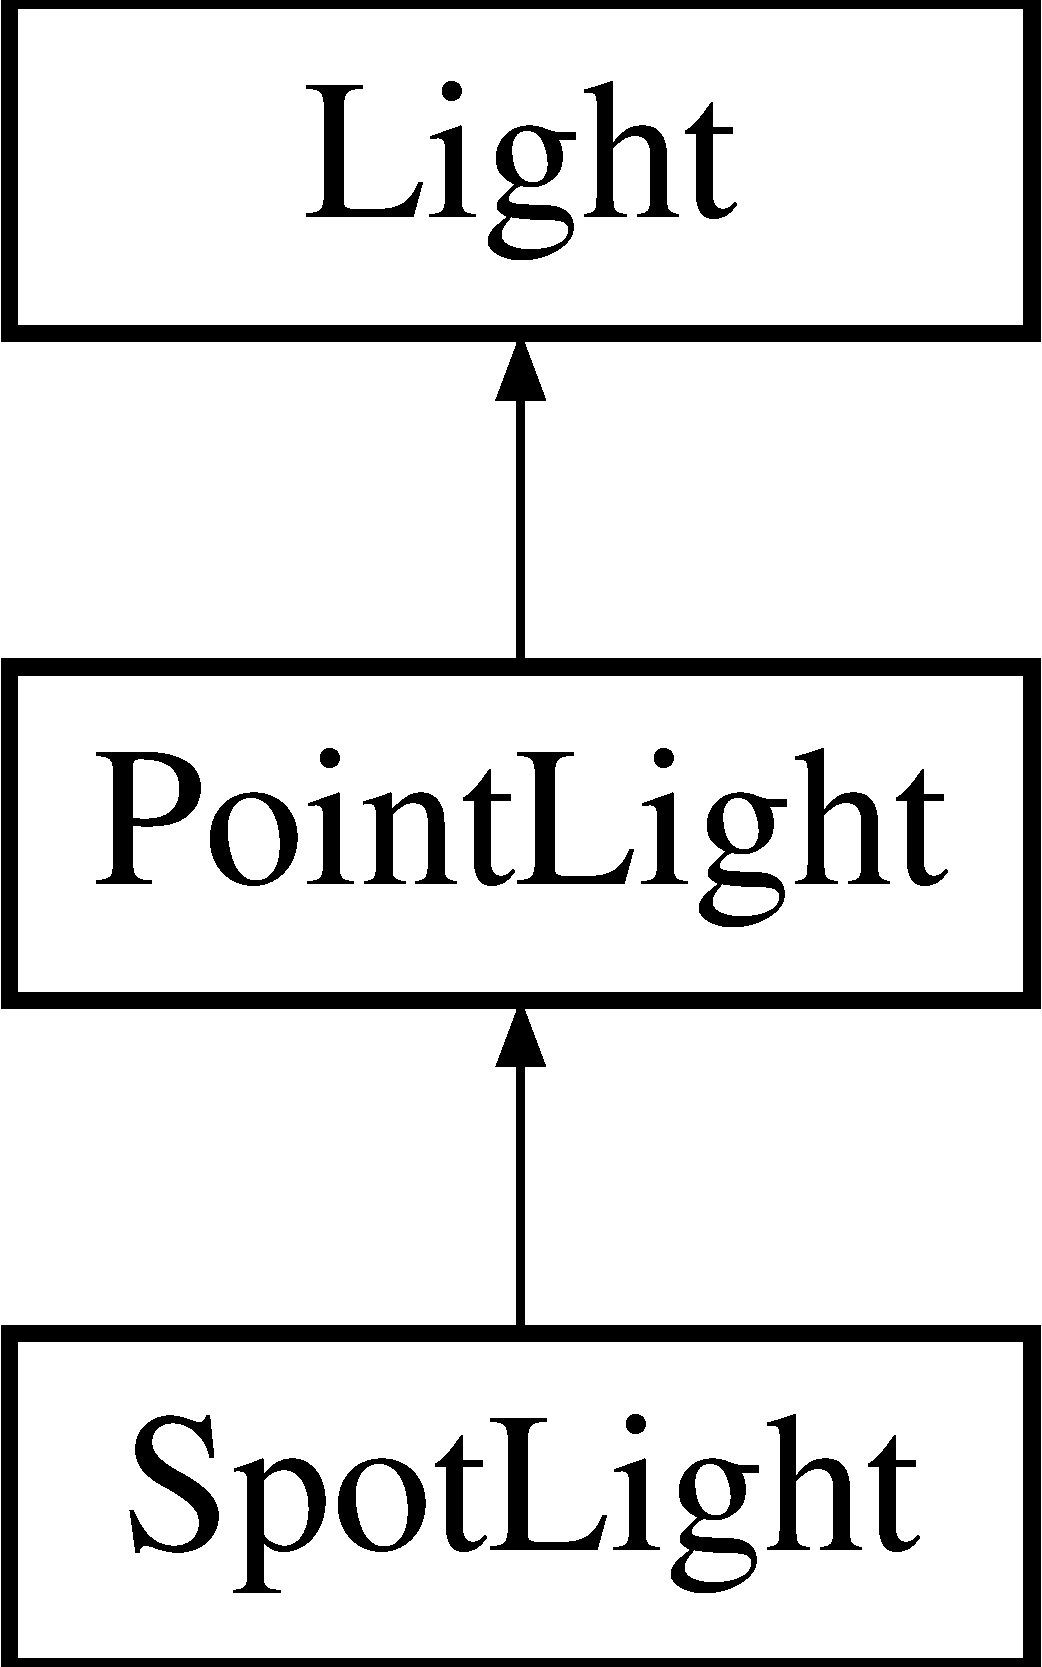
\includegraphics[height=3.000000cm]{classSpotLight}
\end{center}
\end{figure}
\subsection*{Public Member Functions}
\begin{DoxyCompactItemize}
\item 
virtual void \hyperlink{classSpotLight_a4599dbd0a665514ff7066bfa01d04d1e}{set\+Uniforms} (const \hyperlink{classShader}{Shader} \&shader, const std\+::string \&uname) const
\item 
virtual void \hyperlink{classSpotLight_a7ca46a2356ceb4f193704632e1f17bb4}{ui} ()
\end{DoxyCompactItemize}
\subsection*{Public Attributes}
\begin{DoxyCompactItemize}
\item 
float \hyperlink{classSpotLight_a434b4b2ad7072d34e238c529b6376608}{cut\+Off\+\_\+} = 12.\+5f
\item 
float \hyperlink{classSpotLight_aea3df0ad93a03e5a477ac431a394178d}{outer\+Cut\+Off\+\_\+} = 20.f
\item 
glm\+::vec3 \hyperlink{classSpotLight_a55620e0b9baa8ac72dacede2420bf121}{direction\+\_\+} = \{-\/10.f, -\/10.f, -\/10.f\}
\end{DoxyCompactItemize}


\subsection{Member Function Documentation}
\mbox{\Hypertarget{classSpotLight_a4599dbd0a665514ff7066bfa01d04d1e}\label{classSpotLight_a4599dbd0a665514ff7066bfa01d04d1e}} 
\index{Spot\+Light@{Spot\+Light}!set\+Uniforms@{set\+Uniforms}}
\index{set\+Uniforms@{set\+Uniforms}!Spot\+Light@{Spot\+Light}}
\subsubsection{\texorpdfstring{set\+Uniforms()}{setUniforms()}}
{\footnotesize\ttfamily void Spot\+Light\+::set\+Uniforms (\begin{DoxyParamCaption}\item[{const \hyperlink{classShader}{Shader} \&}]{shader,  }\item[{const std\+::string \&}]{uname }\end{DoxyParamCaption}) const\hspace{0.3cm}{\ttfamily [virtual]}}



Reimplemented from \hyperlink{classPointLight_abf6f298a0d04b636e22a3a5903e5b823}{Point\+Light}.

\mbox{\Hypertarget{classSpotLight_a7ca46a2356ceb4f193704632e1f17bb4}\label{classSpotLight_a7ca46a2356ceb4f193704632e1f17bb4}} 
\index{Spot\+Light@{Spot\+Light}!ui@{ui}}
\index{ui@{ui}!Spot\+Light@{Spot\+Light}}
\subsubsection{\texorpdfstring{ui()}{ui()}}
{\footnotesize\ttfamily void Spot\+Light\+::ui (\begin{DoxyParamCaption}{ }\end{DoxyParamCaption})\hspace{0.3cm}{\ttfamily [virtual]}}



Reimplemented from \hyperlink{classPointLight_a538a42e0d1d713c57e46e492d352b34e}{Point\+Light}.



\subsection{Member Data Documentation}
\mbox{\Hypertarget{classSpotLight_a434b4b2ad7072d34e238c529b6376608}\label{classSpotLight_a434b4b2ad7072d34e238c529b6376608}} 
\index{Spot\+Light@{Spot\+Light}!cut\+Off\+\_\+@{cut\+Off\+\_\+}}
\index{cut\+Off\+\_\+@{cut\+Off\+\_\+}!Spot\+Light@{Spot\+Light}}
\subsubsection{\texorpdfstring{cut\+Off\+\_\+}{cutOff\_}}
{\footnotesize\ttfamily float Spot\+Light\+::cut\+Off\+\_\+ = 12.\+5f}

\mbox{\Hypertarget{classSpotLight_a55620e0b9baa8ac72dacede2420bf121}\label{classSpotLight_a55620e0b9baa8ac72dacede2420bf121}} 
\index{Spot\+Light@{Spot\+Light}!direction\+\_\+@{direction\+\_\+}}
\index{direction\+\_\+@{direction\+\_\+}!Spot\+Light@{Spot\+Light}}
\subsubsection{\texorpdfstring{direction\+\_\+}{direction\_}}
{\footnotesize\ttfamily glm\+::vec3 Spot\+Light\+::direction\+\_\+ = \{-\/10.f, -\/10.f, -\/10.f\}}

\mbox{\Hypertarget{classSpotLight_aea3df0ad93a03e5a477ac431a394178d}\label{classSpotLight_aea3df0ad93a03e5a477ac431a394178d}} 
\index{Spot\+Light@{Spot\+Light}!outer\+Cut\+Off\+\_\+@{outer\+Cut\+Off\+\_\+}}
\index{outer\+Cut\+Off\+\_\+@{outer\+Cut\+Off\+\_\+}!Spot\+Light@{Spot\+Light}}
\subsubsection{\texorpdfstring{outer\+Cut\+Off\+\_\+}{outerCutOff\_}}
{\footnotesize\ttfamily float Spot\+Light\+::outer\+Cut\+Off\+\_\+ = 20.f}



The documentation for this class was generated from the following files\+:\begin{DoxyCompactItemize}
\item 
src/\hyperlink{light_8h}{light.\+h}\item 
src/\hyperlink{light_8cpp}{light.\+cpp}\end{DoxyCompactItemize}

\hypertarget{classTerrain}{}\section{Terrain Class Reference}
\label{classTerrain}\index{Terrain@{Terrain}}


A \hyperlink{classTerrain}{Terrain}.  




{\ttfamily \#include $<$terrain.\+h$>$}

Inheritance diagram for Terrain\+:\begin{figure}[H]
\begin{center}
\leavevmode
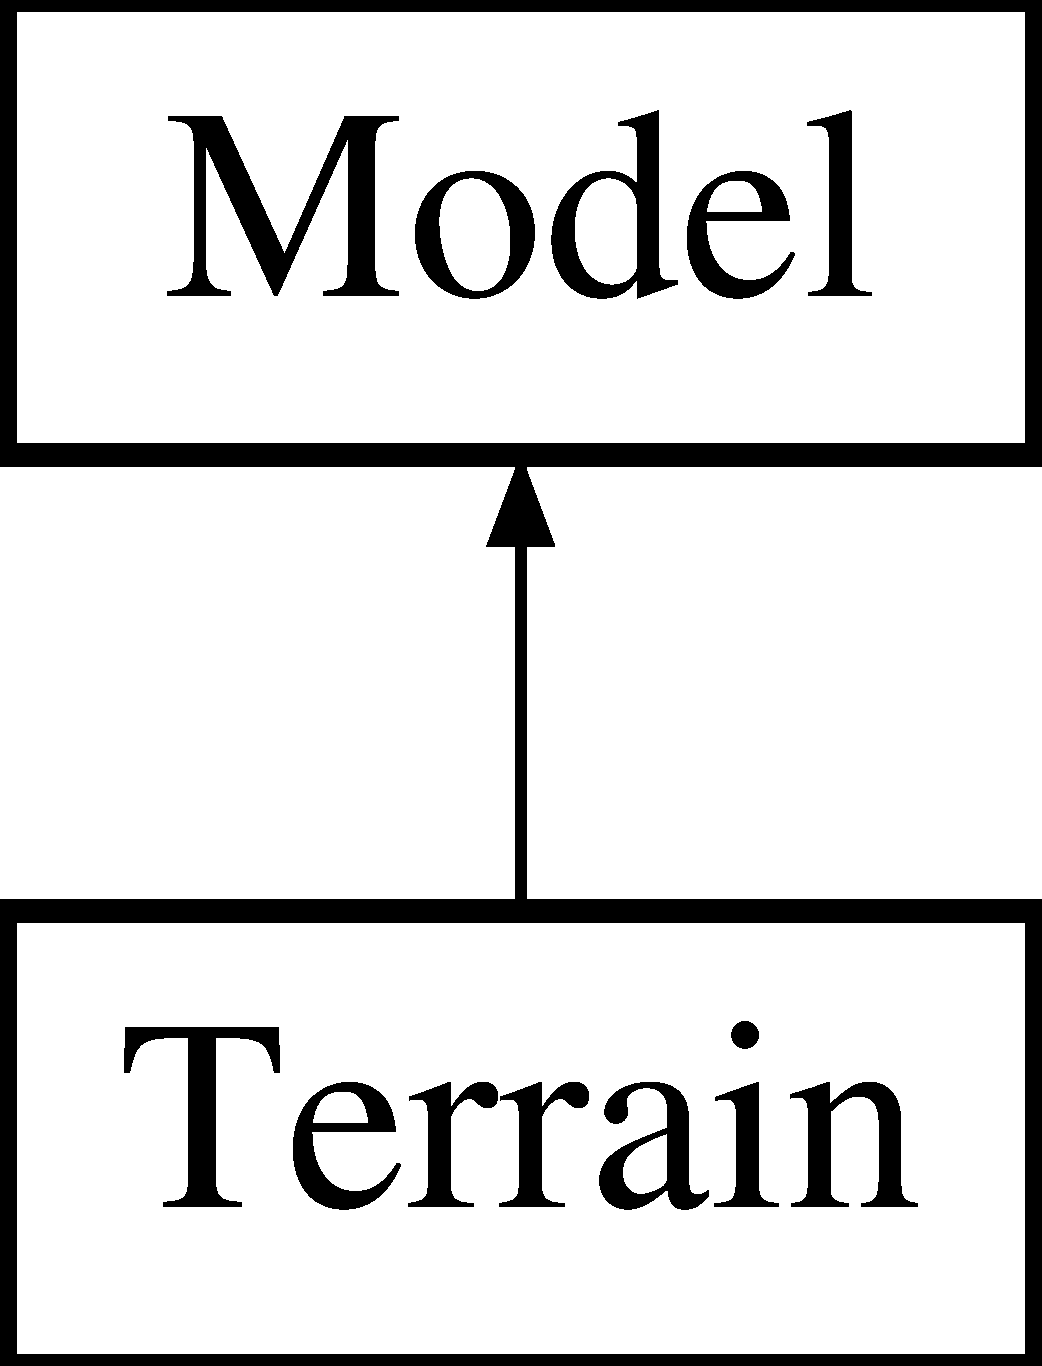
\includegraphics[height=2.000000cm]{classTerrain}
\end{center}
\end{figure}
\subsection*{Public Member Functions}
\begin{DoxyCompactItemize}
\item 
\hyperlink{classTerrain_afafc221c37b67156d8dedeeee5f9f0e5}{Terrain} (const \hyperlink{classGrid}{Grid} \&)
\begin{DoxyCompactList}\small\item\em Generate a terrain from a grid. \end{DoxyCompactList}\item 
void \hyperlink{classTerrain_ac3a615c383f37e7fc9894d20cc090da2}{draw} (const \hyperlink{classShader}{Shader} \&shader)
\begin{DoxyCompactList}\small\item\em Draw the terrain This override set the model mat to nothing. \end{DoxyCompactList}\item 
void \hyperlink{classTerrain_abc478a72ef7b4b9dae3911d1acee4c71}{randomize} ()
\begin{DoxyCompactList}\small\item\em Randomize the height of the terrain using a perlin noise. \end{DoxyCompactList}\item 
void \hyperlink{classTerrain_afff1911e27bd05cf1da59799db595322}{ui} ()
\end{DoxyCompactItemize}
\subsection*{Static Public Member Functions}
\begin{DoxyCompactItemize}
\item 
static void \hyperlink{classTerrain_a9fa2515b7c84025c74c97af9b3fee30f}{randomize} (std\+::vector$<$ \hyperlink{structVertex}{Vertex} $>$ \&p\+Points, unsigned int p\+Slicing)
\begin{DoxyCompactList}\small\item\em Randomize a given set of point. \end{DoxyCompactList}\item 
static void \hyperlink{classTerrain_aa6063c2dfbed2fbba76800687288f24e}{calculate\+Normals} (std\+::vector$<$ \hyperlink{structVertex}{Vertex} $>$ \&, const std\+::vector$<$ unsigned int $>$ \&)
\begin{DoxyCompactList}\small\item\em Calculate normals for the given set of points and given set of triangls. \end{DoxyCompactList}\end{DoxyCompactItemize}
\subsection*{Additional Inherited Members}


\subsection{Detailed Description}
A \hyperlink{classTerrain}{Terrain}. 

\subsection{Constructor \& Destructor Documentation}
\mbox{\Hypertarget{classTerrain_afafc221c37b67156d8dedeeee5f9f0e5}\label{classTerrain_afafc221c37b67156d8dedeeee5f9f0e5}} 
\index{Terrain@{Terrain}!Terrain@{Terrain}}
\index{Terrain@{Terrain}!Terrain@{Terrain}}
\subsubsection{\texorpdfstring{Terrain()}{Terrain()}}
{\footnotesize\ttfamily Terrain\+::\+Terrain (\begin{DoxyParamCaption}\item[{const \hyperlink{classGrid}{Grid} \&}]{p\+Grid }\end{DoxyParamCaption})}



Generate a terrain from a grid. 



\subsection{Member Function Documentation}
\mbox{\Hypertarget{classTerrain_aa6063c2dfbed2fbba76800687288f24e}\label{classTerrain_aa6063c2dfbed2fbba76800687288f24e}} 
\index{Terrain@{Terrain}!calculate\+Normals@{calculate\+Normals}}
\index{calculate\+Normals@{calculate\+Normals}!Terrain@{Terrain}}
\subsubsection{\texorpdfstring{calculate\+Normals()}{calculateNormals()}}
{\footnotesize\ttfamily void Terrain\+::calculate\+Normals (\begin{DoxyParamCaption}\item[{std\+::vector$<$ \hyperlink{structVertex}{Vertex} $>$ \&}]{p\+Points,  }\item[{const std\+::vector$<$ unsigned int $>$ \&}]{p\+Triangles }\end{DoxyParamCaption})\hspace{0.3cm}{\ttfamily [static]}}



Calculate normals for the given set of points and given set of triangls. 


\begin{DoxyParams}{Parameters}
{\em Points} & \\
\hline
{\em Triangle} & indices \\
\hline
\end{DoxyParams}
\mbox{\Hypertarget{classTerrain_ac3a615c383f37e7fc9894d20cc090da2}\label{classTerrain_ac3a615c383f37e7fc9894d20cc090da2}} 
\index{Terrain@{Terrain}!draw@{draw}}
\index{draw@{draw}!Terrain@{Terrain}}
\subsubsection{\texorpdfstring{draw()}{draw()}}
{\footnotesize\ttfamily void Terrain\+::draw (\begin{DoxyParamCaption}\item[{const \hyperlink{classShader}{Shader} \&}]{shader }\end{DoxyParamCaption})\hspace{0.3cm}{\ttfamily [virtual]}}



Draw the terrain This override set the model mat to nothing. 



Reimplemented from \hyperlink{classModel_a125ff27c588f7f9acfc59c20dcc313b2}{Model}.

\mbox{\Hypertarget{classTerrain_abc478a72ef7b4b9dae3911d1acee4c71}\label{classTerrain_abc478a72ef7b4b9dae3911d1acee4c71}} 
\index{Terrain@{Terrain}!randomize@{randomize}}
\index{randomize@{randomize}!Terrain@{Terrain}}
\subsubsection{\texorpdfstring{randomize()}{randomize()}\hspace{0.1cm}{\footnotesize\ttfamily [1/2]}}
{\footnotesize\ttfamily void Terrain\+::randomize (\begin{DoxyParamCaption}{ }\end{DoxyParamCaption})}



Randomize the height of the terrain using a perlin noise. 

\mbox{\Hypertarget{classTerrain_a9fa2515b7c84025c74c97af9b3fee30f}\label{classTerrain_a9fa2515b7c84025c74c97af9b3fee30f}} 
\index{Terrain@{Terrain}!randomize@{randomize}}
\index{randomize@{randomize}!Terrain@{Terrain}}
\subsubsection{\texorpdfstring{randomize()}{randomize()}\hspace{0.1cm}{\footnotesize\ttfamily [2/2]}}
{\footnotesize\ttfamily void Terrain\+::randomize (\begin{DoxyParamCaption}\item[{std\+::vector$<$ \hyperlink{structVertex}{Vertex} $>$ \&}]{p\+Points,  }\item[{unsigned int}]{p\+Slicing }\end{DoxyParamCaption})\hspace{0.3cm}{\ttfamily [static]}}



Randomize a given set of point. 


\begin{DoxyParams}{Parameters}
{\em p\+Points} & \\
\hline
\end{DoxyParams}
\mbox{\Hypertarget{classTerrain_afff1911e27bd05cf1da59799db595322}\label{classTerrain_afff1911e27bd05cf1da59799db595322}} 
\index{Terrain@{Terrain}!ui@{ui}}
\index{ui@{ui}!Terrain@{Terrain}}
\subsubsection{\texorpdfstring{ui()}{ui()}}
{\footnotesize\ttfamily void Terrain\+::ui (\begin{DoxyParamCaption}{ }\end{DoxyParamCaption})\hspace{0.3cm}{\ttfamily [virtual]}}



Reimplemented from \hyperlink{classModel_a6c1d9003a9cb7699ba70b250c69d8ba4}{Model}.



The documentation for this class was generated from the following files\+:\begin{DoxyCompactItemize}
\item 
src/\hyperlink{terrain_8h}{terrain.\+h}\item 
src/\hyperlink{terrain_8cpp}{terrain.\+cpp}\end{DoxyCompactItemize}

\hypertarget{structTexture}{}\section{Texture Struct Reference}
\label{structTexture}\index{Texture@{Texture}}


{\ttfamily \#include $<$mesh.\+h$>$}

\subsection*{Public Attributes}
\begin{DoxyCompactItemize}
\item 
G\+Luint \hyperlink{structTexture_af848138d72c1fc995ab414a71ab10d47}{id}
\item 
std\+::string \hyperlink{structTexture_a916a835d009806f2a57546c7705942b1}{type}
\end{DoxyCompactItemize}


\subsection{Member Data Documentation}
\mbox{\Hypertarget{structTexture_af848138d72c1fc995ab414a71ab10d47}\label{structTexture_af848138d72c1fc995ab414a71ab10d47}} 
\index{Texture@{Texture}!id@{id}}
\index{id@{id}!Texture@{Texture}}
\subsubsection{\texorpdfstring{id}{id}}
{\footnotesize\ttfamily G\+Luint Texture\+::id}

\mbox{\Hypertarget{structTexture_a916a835d009806f2a57546c7705942b1}\label{structTexture_a916a835d009806f2a57546c7705942b1}} 
\index{Texture@{Texture}!type@{type}}
\index{type@{type}!Texture@{Texture}}
\subsubsection{\texorpdfstring{type}{type}}
{\footnotesize\ttfamily std\+::string Texture\+::type}



The documentation for this struct was generated from the following file\+:\begin{DoxyCompactItemize}
\item 
src/\hyperlink{mesh_8h}{mesh.\+h}\end{DoxyCompactItemize}

\hypertarget{classTurtle}{}\section{Turtle Class Reference}
\label{classTurtle}\index{Turtle@{Turtle}}


Unique instance of the main turtle application. Group everything required to make turtle work.  




{\ttfamily \#include $<$turtle.\+h$>$}

\subsection*{Public Member Functions}
\begin{DoxyCompactItemize}
\item 
float \hyperlink{classTurtle_a0dcb4f2259a8f54bdd45988c11ead3c7}{get\+Delta\+Time} () const
\item 
int \hyperlink{classTurtle_ac2be48e2f6b5df9581b0b346038771b3}{get\+Win\+Height} () const
\item 
int \hyperlink{classTurtle_a9e8f4f0b3abafac7b89b118bef6fcaa3}{get\+Win\+Width} () const
\item 
void \hyperlink{classTurtle_a3c5a8cc7cc5a16b3ffb2be0c24eda79c}{init} ()
\begin{DoxyCompactList}\small\item\em Init the application Should be called only once. \end{DoxyCompactList}\item 
void \hyperlink{classTurtle_a42152a0f5631a00428477cbffa8476e1}{terminate} ()
\begin{DoxyCompactList}\small\item\em Correctly terminate the application compounds. Should be called only once. \end{DoxyCompactList}\item 
void \hyperlink{classTurtle_a7f687dce15334de9dbc475ce4869b6c8}{main\+Loop} ()
\begin{DoxyCompactList}\small\item\em Start the main loop which will draw frames. \end{DoxyCompactList}\item 
void \hyperlink{classTurtle_a899c4635a6c30fef7723542e7524f606}{display\+Frame} ()
\begin{DoxyCompactList}\small\item\em Display of frame. \end{DoxyCompactList}\item 
void \hyperlink{classTurtle_a88420dd1ecfc2b1b0d391e153013dc8d}{display\+Lights} ()
\begin{DoxyCompactList}\small\item\em Display world lights. \end{DoxyCompactList}\item 
void \hyperlink{classTurtle_a6150d70ce0dc15374d434be05ea0b75e}{display\+Ui} ()
\begin{DoxyCompactList}\small\item\em Display the ui. Called before each frame contents. \end{DoxyCompactList}\end{DoxyCompactItemize}
\subsection*{Static Public Member Functions}
\begin{DoxyCompactItemize}
\item 
static \hyperlink{classTurtle}{Turtle} \& \hyperlink{classTurtle_aef2d0d0d699166d2de62af68e716757b}{get\+Instance} ()
\begin{DoxyCompactList}\small\item\em Return the instance of the application Create a new one if there isn\textquotesingle{}t any. \end{DoxyCompactList}\end{DoxyCompactItemize}


\subsection{Detailed Description}
Unique instance of the main turtle application. Group everything required to make turtle work. 

\subsection{Member Function Documentation}
\mbox{\Hypertarget{classTurtle_a899c4635a6c30fef7723542e7524f606}\label{classTurtle_a899c4635a6c30fef7723542e7524f606}} 
\index{Turtle@{Turtle}!display\+Frame@{display\+Frame}}
\index{display\+Frame@{display\+Frame}!Turtle@{Turtle}}
\subsubsection{\texorpdfstring{display\+Frame()}{displayFrame()}}
{\footnotesize\ttfamily void Turtle\+::display\+Frame (\begin{DoxyParamCaption}{ }\end{DoxyParamCaption})}



Display of frame. 

\mbox{\Hypertarget{classTurtle_a88420dd1ecfc2b1b0d391e153013dc8d}\label{classTurtle_a88420dd1ecfc2b1b0d391e153013dc8d}} 
\index{Turtle@{Turtle}!display\+Lights@{display\+Lights}}
\index{display\+Lights@{display\+Lights}!Turtle@{Turtle}}
\subsubsection{\texorpdfstring{display\+Lights()}{displayLights()}}
{\footnotesize\ttfamily void Turtle\+::display\+Lights (\begin{DoxyParamCaption}{ }\end{DoxyParamCaption})}



Display world lights. 

\mbox{\Hypertarget{classTurtle_a6150d70ce0dc15374d434be05ea0b75e}\label{classTurtle_a6150d70ce0dc15374d434be05ea0b75e}} 
\index{Turtle@{Turtle}!display\+Ui@{display\+Ui}}
\index{display\+Ui@{display\+Ui}!Turtle@{Turtle}}
\subsubsection{\texorpdfstring{display\+Ui()}{displayUi()}}
{\footnotesize\ttfamily void Turtle\+::display\+Ui (\begin{DoxyParamCaption}{ }\end{DoxyParamCaption})}



Display the ui. Called before each frame contents. 

\mbox{\Hypertarget{classTurtle_a0dcb4f2259a8f54bdd45988c11ead3c7}\label{classTurtle_a0dcb4f2259a8f54bdd45988c11ead3c7}} 
\index{Turtle@{Turtle}!get\+Delta\+Time@{get\+Delta\+Time}}
\index{get\+Delta\+Time@{get\+Delta\+Time}!Turtle@{Turtle}}
\subsubsection{\texorpdfstring{get\+Delta\+Time()}{getDeltaTime()}}
{\footnotesize\ttfamily float Turtle\+::get\+Delta\+Time (\begin{DoxyParamCaption}{ }\end{DoxyParamCaption}) const}

Returns the delta time of the current frame \mbox{\Hypertarget{classTurtle_aef2d0d0d699166d2de62af68e716757b}\label{classTurtle_aef2d0d0d699166d2de62af68e716757b}} 
\index{Turtle@{Turtle}!get\+Instance@{get\+Instance}}
\index{get\+Instance@{get\+Instance}!Turtle@{Turtle}}
\subsubsection{\texorpdfstring{get\+Instance()}{getInstance()}}
{\footnotesize\ttfamily \hyperlink{classTurtle}{Turtle} \& Turtle\+::get\+Instance (\begin{DoxyParamCaption}{ }\end{DoxyParamCaption})\hspace{0.3cm}{\ttfamily [static]}}



Return the instance of the application Create a new one if there isn\textquotesingle{}t any. 

\begin{DoxyReturn}{Returns}

\end{DoxyReturn}
\mbox{\Hypertarget{classTurtle_ac2be48e2f6b5df9581b0b346038771b3}\label{classTurtle_ac2be48e2f6b5df9581b0b346038771b3}} 
\index{Turtle@{Turtle}!get\+Win\+Height@{get\+Win\+Height}}
\index{get\+Win\+Height@{get\+Win\+Height}!Turtle@{Turtle}}
\subsubsection{\texorpdfstring{get\+Win\+Height()}{getWinHeight()}}
{\footnotesize\ttfamily int Turtle\+::get\+Win\+Height (\begin{DoxyParamCaption}{ }\end{DoxyParamCaption}) const}

\mbox{\Hypertarget{classTurtle_a9e8f4f0b3abafac7b89b118bef6fcaa3}\label{classTurtle_a9e8f4f0b3abafac7b89b118bef6fcaa3}} 
\index{Turtle@{Turtle}!get\+Win\+Width@{get\+Win\+Width}}
\index{get\+Win\+Width@{get\+Win\+Width}!Turtle@{Turtle}}
\subsubsection{\texorpdfstring{get\+Win\+Width()}{getWinWidth()}}
{\footnotesize\ttfamily int Turtle\+::get\+Win\+Width (\begin{DoxyParamCaption}{ }\end{DoxyParamCaption}) const}

\mbox{\Hypertarget{classTurtle_a3c5a8cc7cc5a16b3ffb2be0c24eda79c}\label{classTurtle_a3c5a8cc7cc5a16b3ffb2be0c24eda79c}} 
\index{Turtle@{Turtle}!init@{init}}
\index{init@{init}!Turtle@{Turtle}}
\subsubsection{\texorpdfstring{init()}{init()}}
{\footnotesize\ttfamily void Turtle\+::init (\begin{DoxyParamCaption}{ }\end{DoxyParamCaption})}



Init the application Should be called only once. 

\mbox{\Hypertarget{classTurtle_a7f687dce15334de9dbc475ce4869b6c8}\label{classTurtle_a7f687dce15334de9dbc475ce4869b6c8}} 
\index{Turtle@{Turtle}!main\+Loop@{main\+Loop}}
\index{main\+Loop@{main\+Loop}!Turtle@{Turtle}}
\subsubsection{\texorpdfstring{main\+Loop()}{mainLoop()}}
{\footnotesize\ttfamily void Turtle\+::main\+Loop (\begin{DoxyParamCaption}{ }\end{DoxyParamCaption})}



Start the main loop which will draw frames. 

\mbox{\Hypertarget{classTurtle_a42152a0f5631a00428477cbffa8476e1}\label{classTurtle_a42152a0f5631a00428477cbffa8476e1}} 
\index{Turtle@{Turtle}!terminate@{terminate}}
\index{terminate@{terminate}!Turtle@{Turtle}}
\subsubsection{\texorpdfstring{terminate()}{terminate()}}
{\footnotesize\ttfamily void Turtle\+::terminate (\begin{DoxyParamCaption}{ }\end{DoxyParamCaption})}



Correctly terminate the application compounds. Should be called only once. 



The documentation for this class was generated from the following files\+:\begin{DoxyCompactItemize}
\item 
src/\hyperlink{turtle_8h}{turtle.\+h}\item 
src/\hyperlink{turtle_8cpp}{turtle.\+cpp}\end{DoxyCompactItemize}

\hypertarget{structVertex}{}\section{Vertex Struct Reference}
\label{structVertex}\index{Vertex@{Vertex}}


{\ttfamily \#include $<$mesh.\+h$>$}

\subsection*{Public Attributes}
\begin{DoxyCompactItemize}
\item 
glm\+::vec3 \hyperlink{structVertex_abb3cfacd96b5955b0cec9359840ee49f}{Position}
\item 
glm\+::vec3 \hyperlink{structVertex_a9ab4dc431b41509f0b1bb1a4bf09d4e2}{Normal}
\item 
glm\+::vec3 \hyperlink{structVertex_a559b1c0085e92418f4604bfbd0cf7364}{Tex\+Coords}
\end{DoxyCompactItemize}


\subsection{Member Data Documentation}
\mbox{\Hypertarget{structVertex_a9ab4dc431b41509f0b1bb1a4bf09d4e2}\label{structVertex_a9ab4dc431b41509f0b1bb1a4bf09d4e2}} 
\index{Vertex@{Vertex}!Normal@{Normal}}
\index{Normal@{Normal}!Vertex@{Vertex}}
\subsubsection{\texorpdfstring{Normal}{Normal}}
{\footnotesize\ttfamily glm\+::vec3 Vertex\+::\+Normal}

\mbox{\Hypertarget{structVertex_abb3cfacd96b5955b0cec9359840ee49f}\label{structVertex_abb3cfacd96b5955b0cec9359840ee49f}} 
\index{Vertex@{Vertex}!Position@{Position}}
\index{Position@{Position}!Vertex@{Vertex}}
\subsubsection{\texorpdfstring{Position}{Position}}
{\footnotesize\ttfamily glm\+::vec3 Vertex\+::\+Position}

\mbox{\Hypertarget{structVertex_a559b1c0085e92418f4604bfbd0cf7364}\label{structVertex_a559b1c0085e92418f4604bfbd0cf7364}} 
\index{Vertex@{Vertex}!Tex\+Coords@{Tex\+Coords}}
\index{Tex\+Coords@{Tex\+Coords}!Vertex@{Vertex}}
\subsubsection{\texorpdfstring{Tex\+Coords}{TexCoords}}
{\footnotesize\ttfamily glm\+::vec3 Vertex\+::\+Tex\+Coords}



The documentation for this struct was generated from the following file\+:\begin{DoxyCompactItemize}
\item 
src/\hyperlink{mesh_8h}{mesh.\+h}\end{DoxyCompactItemize}

\chapter{File Documentation}
\hypertarget{camera_8cpp}{}\section{src/camera.cpp File Reference}
\label{camera_8cpp}\index{src/camera.\+cpp@{src/camera.\+cpp}}
{\ttfamily \#include \char`\"{}camera.\+h\char`\"{}}\newline
{\ttfamily \#include \char`\"{}turtle.\+h\char`\"{}}\newline

\hypertarget{camera_8h}{}\section{src/camera.h File Reference}
\label{camera_8h}\index{src/camera.\+h@{src/camera.\+h}}
{\ttfamily \#include $<$glm/glm.\+hpp$>$}\newline
{\ttfamily \#include $<$glm/gtc/type\+\_\+ptr.\+hpp$>$}\newline
{\ttfamily \#include $<$glm/gtc/matrix\+\_\+transform.\+hpp$>$}\newline
{\ttfamily \#include $<$glm/gtx/rotate\+\_\+vector.\+hpp$>$}\newline
{\ttfamily \#include $<$G\+L/gl3w.\+h$>$}\newline
{\ttfamily \#include $<$G\+L\+F\+W/glfw3.\+h$>$}\newline
\subsection*{Classes}
\begin{DoxyCompactItemize}
\item 
class \hyperlink{classCamera}{Camera}
\begin{DoxyCompactList}\small\item\em \hyperlink{classCamera}{Camera} used to navigate in a scene. \end{DoxyCompactList}\end{DoxyCompactItemize}

\hypertarget{fpsCamera_8cpp}{}\section{src/fps\+Camera.cpp File Reference}
\label{fpsCamera_8cpp}\index{src/fps\+Camera.\+cpp@{src/fps\+Camera.\+cpp}}
{\ttfamily \#include \char`\"{}fps\+Camera.\+h\char`\"{}}\newline
{\ttfamily \#include \char`\"{}turtle.\+h\char`\"{}}\newline

\hypertarget{fpsCamera_8h}{}\section{src/fps\+Camera.h File Reference}
\label{fpsCamera_8h}\index{src/fps\+Camera.\+h@{src/fps\+Camera.\+h}}
{\ttfamily \#include \char`\"{}camera.\+h\char`\"{}}\newline
\subsection*{Classes}
\begin{DoxyCompactItemize}
\item 
class \hyperlink{classFPSCamera}{F\+P\+S\+Camera}
\begin{DoxyCompactList}\small\item\em \hyperlink{classCamera}{Camera} used to navigate in a scene. \end{DoxyCompactList}\end{DoxyCompactItemize}

\hypertarget{grid_8cpp}{}\section{src/grid.cpp File Reference}
\label{grid_8cpp}\index{src/grid.\+cpp@{src/grid.\+cpp}}
{\ttfamily \#include \char`\"{}grid.\+h\char`\"{}}\newline

\hypertarget{grid_8h}{}\section{src/grid.h File Reference}
\label{grid_8h}\index{src/grid.\+h@{src/grid.\+h}}
{\ttfamily \#include $<$glm/vec2.\+hpp$>$}\newline
{\ttfamily \#include $<$vector$>$}\newline
\subsection*{Classes}
\begin{DoxyCompactItemize}
\item 
class \hyperlink{classGrid}{Grid}
\begin{DoxyCompactList}\small\item\em A point grid. \end{DoxyCompactList}\item 
class \hyperlink{classGridGenerator}{Grid\+Generator}
\begin{DoxyCompactList}\small\item\em \hyperlink{classGrid}{Grid} generator. \end{DoxyCompactList}\end{DoxyCompactItemize}

\hypertarget{light_8cpp}{}\section{src/light.cpp File Reference}
\label{light_8cpp}\index{src/light.\+cpp@{src/light.\+cpp}}
{\ttfamily \#include $<$imgui.\+h$>$}\newline
{\ttfamily \#include $<$glm/gtc/type\+\_\+ptr.\+hpp$>$}\newline
{\ttfamily \#include \char`\"{}light.\+h\char`\"{}}\newline

\hypertarget{light_8h}{}\section{src/light.h File Reference}
\label{light_8h}\index{src/light.\+h@{src/light.\+h}}
{\ttfamily \#include $<$string$>$}\newline
{\ttfamily \#include $<$glm/glm.\+hpp$>$}\newline
{\ttfamily \#include \char`\"{}shader.\+h\char`\"{}}\newline
\subsection*{Classes}
\begin{DoxyCompactItemize}
\item 
class \hyperlink{classLight}{Light}
\item 
class \hyperlink{classDirectionLight}{Direction\+Light}
\item 
class \hyperlink{classPointLight}{Point\+Light}
\item 
class \hyperlink{classSpotLight}{Spot\+Light}
\end{DoxyCompactItemize}

\hypertarget{main_8cpp}{}\section{src/main.cpp File Reference}
\label{main_8cpp}\index{src/main.\+cpp@{src/main.\+cpp}}
{\ttfamily \#include $<$iostream$>$}\newline
{\ttfamily \#include $<$string$>$}\newline
{\ttfamily \#include \char`\"{}stb\+\_\+image.\+h\char`\"{}}\newline
{\ttfamily \#include \char`\"{}turtle.\+h\char`\"{}}\newline
{\ttfamily \#include $<$assimp/\+Importer.\+hpp$>$}\newline
{\ttfamily \#include $<$assimp/scene.\+h$>$}\newline
{\ttfamily \#include $<$assimp/material.\+h$>$}\newline
{\ttfamily \#include $<$assimp/postprocess.\+h$>$}\newline
\subsection*{Macros}
\begin{DoxyCompactItemize}
\item 
\#define \hyperlink{main_8cpp_a18372412ad2fc3ce1e3240b3cf0efe78}{S\+T\+B\+\_\+\+I\+M\+A\+G\+E\+\_\+\+I\+M\+P\+L\+E\+M\+E\+N\+T\+A\+T\+I\+ON}
\end{DoxyCompactItemize}
\subsection*{Functions}
\begin{DoxyCompactItemize}
\item 
int \hyperlink{main_8cpp_ae66f6b31b5ad750f1fe042a706a4e3d4}{main} ()
\end{DoxyCompactItemize}


\subsection{Macro Definition Documentation}
\mbox{\Hypertarget{main_8cpp_a18372412ad2fc3ce1e3240b3cf0efe78}\label{main_8cpp_a18372412ad2fc3ce1e3240b3cf0efe78}} 
\index{main.\+cpp@{main.\+cpp}!S\+T\+B\+\_\+\+I\+M\+A\+G\+E\+\_\+\+I\+M\+P\+L\+E\+M\+E\+N\+T\+A\+T\+I\+ON@{S\+T\+B\+\_\+\+I\+M\+A\+G\+E\+\_\+\+I\+M\+P\+L\+E\+M\+E\+N\+T\+A\+T\+I\+ON}}
\index{S\+T\+B\+\_\+\+I\+M\+A\+G\+E\+\_\+\+I\+M\+P\+L\+E\+M\+E\+N\+T\+A\+T\+I\+ON@{S\+T\+B\+\_\+\+I\+M\+A\+G\+E\+\_\+\+I\+M\+P\+L\+E\+M\+E\+N\+T\+A\+T\+I\+ON}!main.\+cpp@{main.\+cpp}}
\subsubsection{\texorpdfstring{S\+T\+B\+\_\+\+I\+M\+A\+G\+E\+\_\+\+I\+M\+P\+L\+E\+M\+E\+N\+T\+A\+T\+I\+ON}{STB\_IMAGE\_IMPLEMENTATION}}
{\footnotesize\ttfamily \#define S\+T\+B\+\_\+\+I\+M\+A\+G\+E\+\_\+\+I\+M\+P\+L\+E\+M\+E\+N\+T\+A\+T\+I\+ON}



\subsection{Function Documentation}
\mbox{\Hypertarget{main_8cpp_ae66f6b31b5ad750f1fe042a706a4e3d4}\label{main_8cpp_ae66f6b31b5ad750f1fe042a706a4e3d4}} 
\index{main.\+cpp@{main.\+cpp}!main@{main}}
\index{main@{main}!main.\+cpp@{main.\+cpp}}
\subsubsection{\texorpdfstring{main()}{main()}}
{\footnotesize\ttfamily int main (\begin{DoxyParamCaption}{ }\end{DoxyParamCaption})}


\hypertarget{mesh_8cpp}{}\section{src/mesh.cpp File Reference}
\label{mesh_8cpp}\index{src/mesh.\+cpp@{src/mesh.\+cpp}}
{\ttfamily \#include \char`\"{}mesh.\+h\char`\"{}}\newline
{\ttfamily \#include $<$stdexcept$>$}\newline
{\ttfamily \#include $<$iostream$>$}\newline

\hypertarget{mesh_8h}{}\section{src/mesh.h File Reference}
\label{mesh_8h}\index{src/mesh.\+h@{src/mesh.\+h}}
{\ttfamily \#include \char`\"{}shader.\+h\char`\"{}}\newline
{\ttfamily \#include $<$vector$>$}\newline
{\ttfamily \#include $<$assimp/\+Importer.\+hpp$>$}\newline
{\ttfamily \#include $<$G\+L/gl3w.\+h$>$}\newline
{\ttfamily \#include $<$G\+L\+F\+W/glfw3.\+h$>$}\newline
{\ttfamily \#include $<$glm/glm.\+hpp$>$}\newline
{\ttfamily \#include $<$glm/gtc/matrix\+\_\+transform.\+hpp$>$}\newline
\subsection*{Classes}
\begin{DoxyCompactItemize}
\item 
struct \hyperlink{structVertex}{Vertex}
\item 
struct \hyperlink{structTexture}{Texture}
\item 
class \hyperlink{classMesh}{Mesh}
\begin{DoxyCompactList}\small\item\em \hyperlink{classMesh}{Mesh} wrapper. \end{DoxyCompactList}\end{DoxyCompactItemize}

\hypertarget{model_8cpp}{}\section{src/model.cpp File Reference}
\label{model_8cpp}\index{src/model.\+cpp@{src/model.\+cpp}}
{\ttfamily \#include \char`\"{}model.\+h\char`\"{}}\newline
{\ttfamily \#include $<$list$>$}\newline
{\ttfamily \#include $<$glm/gtc/matrix\+\_\+transform.\+hpp$>$}\newline
{\ttfamily \#include $<$glm/gtc/type\+\_\+ptr.\+hpp$>$}\newline
{\ttfamily \#include $<$imgui.\+h$>$}\newline
{\ttfamily \#include \char`\"{}stb\+\_\+image.\+h\char`\"{}}\newline
\subsection*{Functions}
\begin{DoxyCompactItemize}
\item 
G\+Luint \hyperlink{model_8cpp_aaca61c1ab52f5a6c7613231957c15936}{texture\+From\+File} (const char $\ast$path, const std\+::string \&directory, bool gamma)
\end{DoxyCompactItemize}


\subsection{Function Documentation}
\mbox{\Hypertarget{model_8cpp_aaca61c1ab52f5a6c7613231957c15936}\label{model_8cpp_aaca61c1ab52f5a6c7613231957c15936}} 
\index{model.\+cpp@{model.\+cpp}!texture\+From\+File@{texture\+From\+File}}
\index{texture\+From\+File@{texture\+From\+File}!model.\+cpp@{model.\+cpp}}
\subsubsection{\texorpdfstring{texture\+From\+File()}{textureFromFile()}}
{\footnotesize\ttfamily G\+Luint texture\+From\+File (\begin{DoxyParamCaption}\item[{const char $\ast$}]{path,  }\item[{const std\+::string \&}]{directory,  }\item[{bool}]{gamma }\end{DoxyParamCaption})}


\hypertarget{model_8h}{}\section{src/model.h File Reference}
\label{model_8h}\index{src/model.\+h@{src/model.\+h}}
{\ttfamily \#include \char`\"{}shader.\+h\char`\"{}}\newline
{\ttfamily \#include \char`\"{}mesh.\+h\char`\"{}}\newline
{\ttfamily \#include $<$string$>$}\newline
{\ttfamily \#include $<$vector$>$}\newline
{\ttfamily \#include $<$assimp/\+Importer.\+hpp$>$}\newline
{\ttfamily \#include $<$assimp/scene.\+h$>$}\newline
{\ttfamily \#include $<$assimp/material.\+h$>$}\newline
{\ttfamily \#include $<$assimp/postprocess.\+h$>$}\newline
\subsection*{Classes}
\begin{DoxyCompactItemize}
\item 
class \hyperlink{classModel}{Model}
\begin{DoxyCompactList}\small\item\em A set of one or more mesh. \end{DoxyCompactList}\end{DoxyCompactItemize}
\subsection*{Functions}
\begin{DoxyCompactItemize}
\item 
G\+Luint \hyperlink{model_8h_a2a935db559df167899a6bf8a86963d9c}{texture\+From\+File} (const char $\ast$path, const std\+::string \&directory, bool gamma=false)
\end{DoxyCompactItemize}


\subsection{Function Documentation}
\mbox{\Hypertarget{model_8h_a2a935db559df167899a6bf8a86963d9c}\label{model_8h_a2a935db559df167899a6bf8a86963d9c}} 
\index{model.\+h@{model.\+h}!texture\+From\+File@{texture\+From\+File}}
\index{texture\+From\+File@{texture\+From\+File}!model.\+h@{model.\+h}}
\subsubsection{\texorpdfstring{texture\+From\+File()}{textureFromFile()}}
{\footnotesize\ttfamily G\+Luint texture\+From\+File (\begin{DoxyParamCaption}\item[{const char $\ast$}]{path,  }\item[{const std\+::string \&}]{directory,  }\item[{bool}]{gamma = {\ttfamily false} }\end{DoxyParamCaption})}


\hypertarget{object_8cpp}{}\section{src/object.cpp File Reference}
\label{object_8cpp}\index{src/object.\+cpp@{src/object.\+cpp}}
{\ttfamily \#include \char`\"{}object.\+h\char`\"{}}\newline
{\ttfamily \#include $<$glm/gtc/matrix\+\_\+transform.\+hpp$>$}\newline
{\ttfamily \#include $<$imgui.\+h$>$}\newline

\hypertarget{object_8h}{}\section{src/object.h File Reference}
\label{object_8h}\index{src/object.\+h@{src/object.\+h}}
{\ttfamily \#include $<$chrono$>$}\newline
{\ttfamily \#include $<$memory$>$}\newline
{\ttfamily \#include $<$random$>$}\newline
{\ttfamily \#include $<$glm/gtc/type\+\_\+ptr.\+hpp$>$}\newline
{\ttfamily \#include \char`\"{}model.\+h\char`\"{}}\newline
{\ttfamily \#include \char`\"{}shader.\+h\char`\"{}}\newline
\subsection*{Classes}
\begin{DoxyCompactItemize}
\item 
class \hyperlink{classObject}{Object}
\begin{DoxyCompactList}\small\item\em Wrapper of a model Can be positioned in the spaces Usefulle when creating instances, avoid to duplicate the model. \end{DoxyCompactList}\end{DoxyCompactItemize}

\hypertarget{orbitCamera_8cpp}{}\section{src/orbit\+Camera.cpp File Reference}
\label{orbitCamera_8cpp}\index{src/orbit\+Camera.\+cpp@{src/orbit\+Camera.\+cpp}}
{\ttfamily \#include \char`\"{}orbit\+Camera.\+h\char`\"{}}\newline
{\ttfamily \#include \char`\"{}turtle.\+h\char`\"{}}\newline

\hypertarget{orbitCamera_8h}{}\section{src/orbit\+Camera.h File Reference}
\label{orbitCamera_8h}\index{src/orbit\+Camera.\+h@{src/orbit\+Camera.\+h}}
{\ttfamily \#include \char`\"{}camera.\+h\char`\"{}}\newline
\subsection*{Classes}
\begin{DoxyCompactItemize}
\item 
class \hyperlink{classOrbitCamera}{Orbit\+Camera}
\begin{DoxyCompactList}\small\item\em \hyperlink{classCamera}{Camera} used to rotate around a round-\/shaped object. \end{DoxyCompactList}\end{DoxyCompactItemize}

\hypertarget{shader_8cpp}{}\section{src/shader.cpp File Reference}
\label{shader_8cpp}\index{src/shader.\+cpp@{src/shader.\+cpp}}
{\ttfamily \#include \char`\"{}shader.\+h\char`\"{}}\newline
{\ttfamily \#include $<$fstream$>$}\newline

\hypertarget{shader_8h}{}\section{src/shader.h File Reference}
\label{shader_8h}\index{src/shader.\+h@{src/shader.\+h}}
{\ttfamily \#include $<$string$>$}\newline
{\ttfamily \#include $<$G\+L/gl3w.\+h$>$}\newline
{\ttfamily \#include $<$G\+L\+F\+W/glfw3.\+h$>$}\newline
{\ttfamily \#include $<$glm/glm.\+hpp$>$}\newline
\subsection*{Classes}
\begin{DoxyCompactItemize}
\item 
class \hyperlink{classShader}{Shader}
\end{DoxyCompactItemize}

\hypertarget{skybox_8cpp}{}\section{src/skybox.cpp File Reference}
\label{skybox_8cpp}\index{src/skybox.\+cpp@{src/skybox.\+cpp}}
{\ttfamily \#include \char`\"{}skybox.\+h\char`\"{}}\newline
{\ttfamily \#include \char`\"{}mesh.\+h\char`\"{}}\newline
{\ttfamily \#include $<$vector$>$}\newline
{\ttfamily \#include \char`\"{}stb\+\_\+image.\+h\char`\"{}}\newline

\hypertarget{skybox_8h}{}\section{src/skybox.h File Reference}
\label{skybox_8h}\index{src/skybox.\+h@{src/skybox.\+h}}
{\ttfamily \#include \char`\"{}shader.\+h\char`\"{}}\newline
{\ttfamily \#include $<$string$>$}\newline
{\ttfamily \#include $<$vector$>$}\newline
\subsection*{Classes}
\begin{DoxyCompactItemize}
\item 
class \hyperlink{classSkyBox}{Sky\+Box}
\begin{DoxyCompactList}\small\item\em A Cubemap. \end{DoxyCompactList}\end{DoxyCompactItemize}

\hypertarget{terrain_8cpp}{}\section{src/terrain.cpp File Reference}
\label{terrain_8cpp}\index{src/terrain.\+cpp@{src/terrain.\+cpp}}
{\ttfamily \#include \char`\"{}terrain.\+h\char`\"{}}\newline
{\ttfamily \#include \char`\"{}Perlin\+Noise.\+h\char`\"{}}\newline
{\ttfamily \#include $<$imgui.\+h$>$}\newline

\hypertarget{terrain_8h}{}\section{src/terrain.h File Reference}
\label{terrain_8h}\index{src/terrain.\+h@{src/terrain.\+h}}
{\ttfamily \#include \char`\"{}grid.\+h\char`\"{}}\newline
{\ttfamily \#include \char`\"{}model.\+h\char`\"{}}\newline
\subsection*{Classes}
\begin{DoxyCompactItemize}
\item 
class \hyperlink{classTerrain}{Terrain}
\begin{DoxyCompactList}\small\item\em A \hyperlink{classTerrain}{Terrain}. \end{DoxyCompactList}\end{DoxyCompactItemize}

\hypertarget{turtle_8cpp}{}\section{src/turtle.cpp File Reference}
\label{turtle_8cpp}\index{src/turtle.\+cpp@{src/turtle.\+cpp}}
{\ttfamily \#include $<$cassert$>$}\newline
{\ttfamily \#include $<$iostream$>$}\newline
{\ttfamily \#include \char`\"{}turtle.\+h\char`\"{}}\newline
{\ttfamily \#include \char`\"{}grid.\+h\char`\"{}}\newline
{\ttfamily \#include \char`\"{}orbit\+Camera.\+h\char`\"{}}\newline
{\ttfamily \#include \char`\"{}fps\+Camera.\+h\char`\"{}}\newline
{\ttfamily \#include \char`\"{}terrain.\+h\char`\"{}}\newline

\hypertarget{turtle_8h}{}\section{src/turtle.h File Reference}
\label{turtle_8h}\index{src/turtle.\+h@{src/turtle.\+h}}
{\ttfamily \#include $<$imgui.\+h$>$}\newline
{\ttfamily \#include \char`\"{}imgui\+\_\+impl\+\_\+glfw\+\_\+gl3.\+h\char`\"{}}\newline
{\ttfamily \#include $<$G\+L/gl3w.\+h$>$}\newline
{\ttfamily \#include $<$G\+L\+F\+W/glfw3.\+h$>$}\newline
{\ttfamily \#include $<$vector$>$}\newline
{\ttfamily \#include $<$map$>$}\newline
{\ttfamily \#include $<$string$>$}\newline
{\ttfamily \#include $<$memory$>$}\newline
{\ttfamily \#include \char`\"{}shader.\+h\char`\"{}}\newline
{\ttfamily \#include \char`\"{}model.\+h\char`\"{}}\newline
{\ttfamily \#include \char`\"{}object.\+h\char`\"{}}\newline
{\ttfamily \#include \char`\"{}terrain.\+h\char`\"{}}\newline
{\ttfamily \#include \char`\"{}camera.\+h\char`\"{}}\newline
{\ttfamily \#include \char`\"{}light.\+h\char`\"{}}\newline
{\ttfamily \#include \char`\"{}skybox.\+h\char`\"{}}\newline
\subsection*{Classes}
\begin{DoxyCompactItemize}
\item 
class \hyperlink{classTurtle}{Turtle}
\begin{DoxyCompactList}\small\item\em Unique instance of the main turtle application. Group everything required to make turtle work. \end{DoxyCompactList}\end{DoxyCompactItemize}

%--- End generated contents ---

% Index
\backmatter
\newpage
\phantomsection
\clearemptydoublepage
\addcontentsline{toc}{chapter}{Index}
\printindex

\end{document}
